
% Default to the notebook output style

    


% Inherit from the specified cell style.




    
\documentclass[11pt]{article}

    
    
    \usepackage[T1]{fontenc}
    % Nicer default font (+ math font) than Computer Modern for most use cases
    \usepackage{mathpazo}

    % Basic figure setup, for now with no caption control since it's done
    % automatically by Pandoc (which extracts ![](path) syntax from Markdown).
    \usepackage{graphicx}
    % We will generate all images so they have a width \maxwidth. This means
    % that they will get their normal width if they fit onto the page, but
    % are scaled down if they would overflow the margins.
    \makeatletter
    \def\maxwidth{\ifdim\Gin@nat@width>\linewidth\linewidth
    \else\Gin@nat@width\fi}
    \makeatother
    \let\Oldincludegraphics\includegraphics
    % Set max figure width to be 80% of text width, for now hardcoded.
    \renewcommand{\includegraphics}[1]{\Oldincludegraphics[width=.8\maxwidth]{#1}}
    % Ensure that by default, figures have no caption (until we provide a
    % proper Figure object with a Caption API and a way to capture that
    % in the conversion process - todo).
    \usepackage{caption}
    \DeclareCaptionLabelFormat{nolabel}{}
    \captionsetup{labelformat=nolabel}

    \usepackage{adjustbox} % Used to constrain images to a maximum size 
    \usepackage{xcolor} % Allow colors to be defined
    \usepackage{enumerate} % Needed for markdown enumerations to work
    \usepackage{geometry} % Used to adjust the document margins
    \usepackage{amsmath} % Equations
    \usepackage{amssymb} % Equations
    \usepackage{textcomp} % defines textquotesingle
    % Hack from http://tex.stackexchange.com/a/47451/13684:
    \AtBeginDocument{%
        \def\PYZsq{\textquotesingle}% Upright quotes in Pygmentized code
    }
    \usepackage{upquote} % Upright quotes for verbatim code
    \usepackage{eurosym} % defines \euro
    \usepackage[mathletters]{ucs} % Extended unicode (utf-8) support
    \usepackage[utf8x]{inputenc} % Allow utf-8 characters in the tex document
    \usepackage{fancyvrb} % verbatim replacement that allows latex
    \usepackage{grffile} % extends the file name processing of package graphics 
                         % to support a larger range 
    % The hyperref package gives us a pdf with properly built
    % internal navigation ('pdf bookmarks' for the table of contents,
    % internal cross-reference links, web links for URLs, etc.)
    \usepackage{hyperref}
    \usepackage{longtable} % longtable support required by pandoc >1.10
    \usepackage{booktabs}  % table support for pandoc > 1.12.2
    \usepackage[inline]{enumitem} % IRkernel/repr support (it uses the enumerate* environment)
    \usepackage[normalem]{ulem} % ulem is needed to support strikethroughs (\sout)
                                % normalem makes italics be italics, not underlines
    

    
    
    % Colors for the hyperref package
    \definecolor{urlcolor}{rgb}{0,.145,.698}
    \definecolor{linkcolor}{rgb}{.71,0.21,0.01}
    \definecolor{citecolor}{rgb}{.12,.54,.11}

    % ANSI colors
    \definecolor{ansi-black}{HTML}{3E424D}
    \definecolor{ansi-black-intense}{HTML}{282C36}
    \definecolor{ansi-red}{HTML}{E75C58}
    \definecolor{ansi-red-intense}{HTML}{B22B31}
    \definecolor{ansi-green}{HTML}{00A250}
    \definecolor{ansi-green-intense}{HTML}{007427}
    \definecolor{ansi-yellow}{HTML}{DDB62B}
    \definecolor{ansi-yellow-intense}{HTML}{B27D12}
    \definecolor{ansi-blue}{HTML}{208FFB}
    \definecolor{ansi-blue-intense}{HTML}{0065CA}
    \definecolor{ansi-magenta}{HTML}{D160C4}
    \definecolor{ansi-magenta-intense}{HTML}{A03196}
    \definecolor{ansi-cyan}{HTML}{60C6C8}
    \definecolor{ansi-cyan-intense}{HTML}{258F8F}
    \definecolor{ansi-white}{HTML}{C5C1B4}
    \definecolor{ansi-white-intense}{HTML}{A1A6B2}

    % commands and environments needed by pandoc snippets
    % extracted from the output of `pandoc -s`
    \providecommand{\tightlist}{%
      \setlength{\itemsep}{0pt}\setlength{\parskip}{0pt}}
    \DefineVerbatimEnvironment{Highlighting}{Verbatim}{commandchars=\\\{\}}
    % Add ',fontsize=\small' for more characters per line
    \newenvironment{Shaded}{}{}
    \newcommand{\KeywordTok}[1]{\textcolor[rgb]{0.00,0.44,0.13}{\textbf{{#1}}}}
    \newcommand{\DataTypeTok}[1]{\textcolor[rgb]{0.56,0.13,0.00}{{#1}}}
    \newcommand{\DecValTok}[1]{\textcolor[rgb]{0.25,0.63,0.44}{{#1}}}
    \newcommand{\BaseNTok}[1]{\textcolor[rgb]{0.25,0.63,0.44}{{#1}}}
    \newcommand{\FloatTok}[1]{\textcolor[rgb]{0.25,0.63,0.44}{{#1}}}
    \newcommand{\CharTok}[1]{\textcolor[rgb]{0.25,0.44,0.63}{{#1}}}
    \newcommand{\StringTok}[1]{\textcolor[rgb]{0.25,0.44,0.63}{{#1}}}
    \newcommand{\CommentTok}[1]{\textcolor[rgb]{0.38,0.63,0.69}{\textit{{#1}}}}
    \newcommand{\OtherTok}[1]{\textcolor[rgb]{0.00,0.44,0.13}{{#1}}}
    \newcommand{\AlertTok}[1]{\textcolor[rgb]{1.00,0.00,0.00}{\textbf{{#1}}}}
    \newcommand{\FunctionTok}[1]{\textcolor[rgb]{0.02,0.16,0.49}{{#1}}}
    \newcommand{\RegionMarkerTok}[1]{{#1}}
    \newcommand{\ErrorTok}[1]{\textcolor[rgb]{1.00,0.00,0.00}{\textbf{{#1}}}}
    \newcommand{\NormalTok}[1]{{#1}}
    
    % Additional commands for more recent versions of Pandoc
    \newcommand{\ConstantTok}[1]{\textcolor[rgb]{0.53,0.00,0.00}{{#1}}}
    \newcommand{\SpecialCharTok}[1]{\textcolor[rgb]{0.25,0.44,0.63}{{#1}}}
    \newcommand{\VerbatimStringTok}[1]{\textcolor[rgb]{0.25,0.44,0.63}{{#1}}}
    \newcommand{\SpecialStringTok}[1]{\textcolor[rgb]{0.73,0.40,0.53}{{#1}}}
    \newcommand{\ImportTok}[1]{{#1}}
    \newcommand{\DocumentationTok}[1]{\textcolor[rgb]{0.73,0.13,0.13}{\textit{{#1}}}}
    \newcommand{\AnnotationTok}[1]{\textcolor[rgb]{0.38,0.63,0.69}{\textbf{\textit{{#1}}}}}
    \newcommand{\CommentVarTok}[1]{\textcolor[rgb]{0.38,0.63,0.69}{\textbf{\textit{{#1}}}}}
    \newcommand{\VariableTok}[1]{\textcolor[rgb]{0.10,0.09,0.49}{{#1}}}
    \newcommand{\ControlFlowTok}[1]{\textcolor[rgb]{0.00,0.44,0.13}{\textbf{{#1}}}}
    \newcommand{\OperatorTok}[1]{\textcolor[rgb]{0.40,0.40,0.40}{{#1}}}
    \newcommand{\BuiltInTok}[1]{{#1}}
    \newcommand{\ExtensionTok}[1]{{#1}}
    \newcommand{\PreprocessorTok}[1]{\textcolor[rgb]{0.74,0.48,0.00}{{#1}}}
    \newcommand{\AttributeTok}[1]{\textcolor[rgb]{0.49,0.56,0.16}{{#1}}}
    \newcommand{\InformationTok}[1]{\textcolor[rgb]{0.38,0.63,0.69}{\textbf{\textit{{#1}}}}}
    \newcommand{\WarningTok}[1]{\textcolor[rgb]{0.38,0.63,0.69}{\textbf{\textit{{#1}}}}}
    
    
    % Define a nice break command that doesn't care if a line doesn't already
    % exist.
    \def\br{\hspace*{\fill} \\* }
    % Math Jax compatability definitions
    \def\gt{>}
    \def\lt{<}
    % Document parameters
    \title{Final Submission}
    
    
    

    % Pygments definitions
    
\makeatletter
\def\PY@reset{\let\PY@it=\relax \let\PY@bf=\relax%
    \let\PY@ul=\relax \let\PY@tc=\relax%
    \let\PY@bc=\relax \let\PY@ff=\relax}
\def\PY@tok#1{\csname PY@tok@#1\endcsname}
\def\PY@toks#1+{\ifx\relax#1\empty\else%
    \PY@tok{#1}\expandafter\PY@toks\fi}
\def\PY@do#1{\PY@bc{\PY@tc{\PY@ul{%
    \PY@it{\PY@bf{\PY@ff{#1}}}}}}}
\def\PY#1#2{\PY@reset\PY@toks#1+\relax+\PY@do{#2}}

\expandafter\def\csname PY@tok@w\endcsname{\def\PY@tc##1{\textcolor[rgb]{0.73,0.73,0.73}{##1}}}
\expandafter\def\csname PY@tok@c\endcsname{\let\PY@it=\textit\def\PY@tc##1{\textcolor[rgb]{0.25,0.50,0.50}{##1}}}
\expandafter\def\csname PY@tok@cp\endcsname{\def\PY@tc##1{\textcolor[rgb]{0.74,0.48,0.00}{##1}}}
\expandafter\def\csname PY@tok@k\endcsname{\let\PY@bf=\textbf\def\PY@tc##1{\textcolor[rgb]{0.00,0.50,0.00}{##1}}}
\expandafter\def\csname PY@tok@kp\endcsname{\def\PY@tc##1{\textcolor[rgb]{0.00,0.50,0.00}{##1}}}
\expandafter\def\csname PY@tok@kt\endcsname{\def\PY@tc##1{\textcolor[rgb]{0.69,0.00,0.25}{##1}}}
\expandafter\def\csname PY@tok@o\endcsname{\def\PY@tc##1{\textcolor[rgb]{0.40,0.40,0.40}{##1}}}
\expandafter\def\csname PY@tok@ow\endcsname{\let\PY@bf=\textbf\def\PY@tc##1{\textcolor[rgb]{0.67,0.13,1.00}{##1}}}
\expandafter\def\csname PY@tok@nb\endcsname{\def\PY@tc##1{\textcolor[rgb]{0.00,0.50,0.00}{##1}}}
\expandafter\def\csname PY@tok@nf\endcsname{\def\PY@tc##1{\textcolor[rgb]{0.00,0.00,1.00}{##1}}}
\expandafter\def\csname PY@tok@nc\endcsname{\let\PY@bf=\textbf\def\PY@tc##1{\textcolor[rgb]{0.00,0.00,1.00}{##1}}}
\expandafter\def\csname PY@tok@nn\endcsname{\let\PY@bf=\textbf\def\PY@tc##1{\textcolor[rgb]{0.00,0.00,1.00}{##1}}}
\expandafter\def\csname PY@tok@ne\endcsname{\let\PY@bf=\textbf\def\PY@tc##1{\textcolor[rgb]{0.82,0.25,0.23}{##1}}}
\expandafter\def\csname PY@tok@nv\endcsname{\def\PY@tc##1{\textcolor[rgb]{0.10,0.09,0.49}{##1}}}
\expandafter\def\csname PY@tok@no\endcsname{\def\PY@tc##1{\textcolor[rgb]{0.53,0.00,0.00}{##1}}}
\expandafter\def\csname PY@tok@nl\endcsname{\def\PY@tc##1{\textcolor[rgb]{0.63,0.63,0.00}{##1}}}
\expandafter\def\csname PY@tok@ni\endcsname{\let\PY@bf=\textbf\def\PY@tc##1{\textcolor[rgb]{0.60,0.60,0.60}{##1}}}
\expandafter\def\csname PY@tok@na\endcsname{\def\PY@tc##1{\textcolor[rgb]{0.49,0.56,0.16}{##1}}}
\expandafter\def\csname PY@tok@nt\endcsname{\let\PY@bf=\textbf\def\PY@tc##1{\textcolor[rgb]{0.00,0.50,0.00}{##1}}}
\expandafter\def\csname PY@tok@nd\endcsname{\def\PY@tc##1{\textcolor[rgb]{0.67,0.13,1.00}{##1}}}
\expandafter\def\csname PY@tok@s\endcsname{\def\PY@tc##1{\textcolor[rgb]{0.73,0.13,0.13}{##1}}}
\expandafter\def\csname PY@tok@sd\endcsname{\let\PY@it=\textit\def\PY@tc##1{\textcolor[rgb]{0.73,0.13,0.13}{##1}}}
\expandafter\def\csname PY@tok@si\endcsname{\let\PY@bf=\textbf\def\PY@tc##1{\textcolor[rgb]{0.73,0.40,0.53}{##1}}}
\expandafter\def\csname PY@tok@se\endcsname{\let\PY@bf=\textbf\def\PY@tc##1{\textcolor[rgb]{0.73,0.40,0.13}{##1}}}
\expandafter\def\csname PY@tok@sr\endcsname{\def\PY@tc##1{\textcolor[rgb]{0.73,0.40,0.53}{##1}}}
\expandafter\def\csname PY@tok@ss\endcsname{\def\PY@tc##1{\textcolor[rgb]{0.10,0.09,0.49}{##1}}}
\expandafter\def\csname PY@tok@sx\endcsname{\def\PY@tc##1{\textcolor[rgb]{0.00,0.50,0.00}{##1}}}
\expandafter\def\csname PY@tok@m\endcsname{\def\PY@tc##1{\textcolor[rgb]{0.40,0.40,0.40}{##1}}}
\expandafter\def\csname PY@tok@gh\endcsname{\let\PY@bf=\textbf\def\PY@tc##1{\textcolor[rgb]{0.00,0.00,0.50}{##1}}}
\expandafter\def\csname PY@tok@gu\endcsname{\let\PY@bf=\textbf\def\PY@tc##1{\textcolor[rgb]{0.50,0.00,0.50}{##1}}}
\expandafter\def\csname PY@tok@gd\endcsname{\def\PY@tc##1{\textcolor[rgb]{0.63,0.00,0.00}{##1}}}
\expandafter\def\csname PY@tok@gi\endcsname{\def\PY@tc##1{\textcolor[rgb]{0.00,0.63,0.00}{##1}}}
\expandafter\def\csname PY@tok@gr\endcsname{\def\PY@tc##1{\textcolor[rgb]{1.00,0.00,0.00}{##1}}}
\expandafter\def\csname PY@tok@ge\endcsname{\let\PY@it=\textit}
\expandafter\def\csname PY@tok@gs\endcsname{\let\PY@bf=\textbf}
\expandafter\def\csname PY@tok@gp\endcsname{\let\PY@bf=\textbf\def\PY@tc##1{\textcolor[rgb]{0.00,0.00,0.50}{##1}}}
\expandafter\def\csname PY@tok@go\endcsname{\def\PY@tc##1{\textcolor[rgb]{0.53,0.53,0.53}{##1}}}
\expandafter\def\csname PY@tok@gt\endcsname{\def\PY@tc##1{\textcolor[rgb]{0.00,0.27,0.87}{##1}}}
\expandafter\def\csname PY@tok@err\endcsname{\def\PY@bc##1{\setlength{\fboxsep}{0pt}\fcolorbox[rgb]{1.00,0.00,0.00}{1,1,1}{\strut ##1}}}
\expandafter\def\csname PY@tok@kc\endcsname{\let\PY@bf=\textbf\def\PY@tc##1{\textcolor[rgb]{0.00,0.50,0.00}{##1}}}
\expandafter\def\csname PY@tok@kd\endcsname{\let\PY@bf=\textbf\def\PY@tc##1{\textcolor[rgb]{0.00,0.50,0.00}{##1}}}
\expandafter\def\csname PY@tok@kn\endcsname{\let\PY@bf=\textbf\def\PY@tc##1{\textcolor[rgb]{0.00,0.50,0.00}{##1}}}
\expandafter\def\csname PY@tok@kr\endcsname{\let\PY@bf=\textbf\def\PY@tc##1{\textcolor[rgb]{0.00,0.50,0.00}{##1}}}
\expandafter\def\csname PY@tok@bp\endcsname{\def\PY@tc##1{\textcolor[rgb]{0.00,0.50,0.00}{##1}}}
\expandafter\def\csname PY@tok@fm\endcsname{\def\PY@tc##1{\textcolor[rgb]{0.00,0.00,1.00}{##1}}}
\expandafter\def\csname PY@tok@vc\endcsname{\def\PY@tc##1{\textcolor[rgb]{0.10,0.09,0.49}{##1}}}
\expandafter\def\csname PY@tok@vg\endcsname{\def\PY@tc##1{\textcolor[rgb]{0.10,0.09,0.49}{##1}}}
\expandafter\def\csname PY@tok@vi\endcsname{\def\PY@tc##1{\textcolor[rgb]{0.10,0.09,0.49}{##1}}}
\expandafter\def\csname PY@tok@vm\endcsname{\def\PY@tc##1{\textcolor[rgb]{0.10,0.09,0.49}{##1}}}
\expandafter\def\csname PY@tok@sa\endcsname{\def\PY@tc##1{\textcolor[rgb]{0.73,0.13,0.13}{##1}}}
\expandafter\def\csname PY@tok@sb\endcsname{\def\PY@tc##1{\textcolor[rgb]{0.73,0.13,0.13}{##1}}}
\expandafter\def\csname PY@tok@sc\endcsname{\def\PY@tc##1{\textcolor[rgb]{0.73,0.13,0.13}{##1}}}
\expandafter\def\csname PY@tok@dl\endcsname{\def\PY@tc##1{\textcolor[rgb]{0.73,0.13,0.13}{##1}}}
\expandafter\def\csname PY@tok@s2\endcsname{\def\PY@tc##1{\textcolor[rgb]{0.73,0.13,0.13}{##1}}}
\expandafter\def\csname PY@tok@sh\endcsname{\def\PY@tc##1{\textcolor[rgb]{0.73,0.13,0.13}{##1}}}
\expandafter\def\csname PY@tok@s1\endcsname{\def\PY@tc##1{\textcolor[rgb]{0.73,0.13,0.13}{##1}}}
\expandafter\def\csname PY@tok@mb\endcsname{\def\PY@tc##1{\textcolor[rgb]{0.40,0.40,0.40}{##1}}}
\expandafter\def\csname PY@tok@mf\endcsname{\def\PY@tc##1{\textcolor[rgb]{0.40,0.40,0.40}{##1}}}
\expandafter\def\csname PY@tok@mh\endcsname{\def\PY@tc##1{\textcolor[rgb]{0.40,0.40,0.40}{##1}}}
\expandafter\def\csname PY@tok@mi\endcsname{\def\PY@tc##1{\textcolor[rgb]{0.40,0.40,0.40}{##1}}}
\expandafter\def\csname PY@tok@il\endcsname{\def\PY@tc##1{\textcolor[rgb]{0.40,0.40,0.40}{##1}}}
\expandafter\def\csname PY@tok@mo\endcsname{\def\PY@tc##1{\textcolor[rgb]{0.40,0.40,0.40}{##1}}}
\expandafter\def\csname PY@tok@ch\endcsname{\let\PY@it=\textit\def\PY@tc##1{\textcolor[rgb]{0.25,0.50,0.50}{##1}}}
\expandafter\def\csname PY@tok@cm\endcsname{\let\PY@it=\textit\def\PY@tc##1{\textcolor[rgb]{0.25,0.50,0.50}{##1}}}
\expandafter\def\csname PY@tok@cpf\endcsname{\let\PY@it=\textit\def\PY@tc##1{\textcolor[rgb]{0.25,0.50,0.50}{##1}}}
\expandafter\def\csname PY@tok@c1\endcsname{\let\PY@it=\textit\def\PY@tc##1{\textcolor[rgb]{0.25,0.50,0.50}{##1}}}
\expandafter\def\csname PY@tok@cs\endcsname{\let\PY@it=\textit\def\PY@tc##1{\textcolor[rgb]{0.25,0.50,0.50}{##1}}}

\def\PYZbs{\char`\\}
\def\PYZus{\char`\_}
\def\PYZob{\char`\{}
\def\PYZcb{\char`\}}
\def\PYZca{\char`\^}
\def\PYZam{\char`\&}
\def\PYZlt{\char`\<}
\def\PYZgt{\char`\>}
\def\PYZsh{\char`\#}
\def\PYZpc{\char`\%}
\def\PYZdl{\char`\$}
\def\PYZhy{\char`\-}
\def\PYZsq{\char`\'}
\def\PYZdq{\char`\"}
\def\PYZti{\char`\~}
% for compatibility with earlier versions
\def\PYZat{@}
\def\PYZlb{[}
\def\PYZrb{]}
\makeatother


    % Exact colors from NB
    \definecolor{incolor}{rgb}{0.0, 0.0, 0.5}
    \definecolor{outcolor}{rgb}{0.545, 0.0, 0.0}



    
    % Prevent overflowing lines due to hard-to-break entities
    \sloppy 
    % Setup hyperref package
    \hypersetup{
      breaklinks=true,  % so long urls are correctly broken across lines
      colorlinks=true,
      urlcolor=urlcolor,
      linkcolor=linkcolor,
      citecolor=citecolor,
      }
    % Slightly bigger margins than the latex defaults
    
    \geometry{verbose,tmargin=1in,bmargin=1in,lmargin=1in,rmargin=1in}
    
    

    \begin{document}
    
    
    \maketitle
    
    

    ---
title: "Diversification Under Market Inefficiency, an NLP Approach"

author:
- Robert Brink
- Marcus Gawronsky
- Christpher Kleyweg
- Ryan Kruger

date: 19 September 2018

abstract: A recent topic of interest in the realm of financial research has been the use of Artificial Intelligence (AI) in financial prediction. This paper explores the use of various techniques in the realm of Natural Language Processing (NLP), using a popular computational technique in deriving meaning from text data, to analyze the relationship between company association and portfolio diversification for companies on the Johannesburg Stock Exchange (JSE). Using a novel take on the Word2Vec word embedding technique, we show word-vector association between companies to track portfolio volatility over time. 

---  
    \newpage

\hypertarget{introduction}{%
\section{Introduction}\label{introduction}}

The Capital Asset Pricing Model (CAPM) remains popular amongst financial
professionals given its simplicity and ease of use. Central to the CAPM
is the assumption of efficient markets, whereby investors are able to
fully diversify away unsystematic risk leaving systematic risk
represented by Beta as the sole risk determinant {[}@Strugnell2011{]}.
However, the concept of perfect diversification prescribed by the CAPM
remains challenging In South Africa or similar markets which exhibit low
forms of efficiency. This leads to an underestimation of risk by South
African investors who may be misled in their investment decisions
through the use of CAPM or its extensions. This paper, therefore,
presents an alternative risk metric known as ``Association Risk'' which
offers investors a way in which to determine the level of
diversification of a given portfolio. This metric is devoid of CAPM
assumptions, using Natural Language Processing (NLP) techniques on
qualitative news articles and analyst reports. This eradicates the
problem of quantitative pricing data which may be unreliable or
corrupted. Portfolios with lower levels of association are shown to be
more diversified, exhibiting lower levels of volatility and therefore
lower levels of risk.

This paper is organized as follows. Section 2 reviews the literature on
the Capital Asset Pricing Model (CAPM) and introduces the use of Natural
Language Processing (NLP) in the financial domain. Section 3 details the
methodology, data, environment and data preprocessing. Section 4
discusses the model specification, benchmarking, experimental design and
method. Section 5 contains the results of this study and is split into
two main sections namely Portfolio ANCOVA and Portfolio ANCOVA with time
blocking. Finally, in Section 6, we summarise and conclude our findings.

\hypertarget{section-2}{%
\section{Section 2}\label{section-2}}

\hypertarget{literature-review}{%
\subsection{Literature Review}\label{literature-review}}

The Capital Asset Pricing Model (CAPM) developed by {[}@Treynor1961,
@Treynor1962, @Sharpe1964, @Lintner1965, @Mossin1966 and @Black1972{]}
remains at the core of modern financial theory by providing investors
with a framework in determining how the expected return of an investment
is affected but its risk {[}@Strugnell2011{]}.

\[ \text{Expected Return} = r_{f} + \beta(r_{m} - r_{f})\]

Where Expected Return is the expected returns of a share in the market,
\(r_{f}\) is the risk-free rate, \(r_{m}\) are the returns of the market
and \(\beta\) is a coefficient computed using through Ordinary Least
Squares Regression, under the assumption of normally distributed errors
{[}@Strugnell2011{]}.

Under CAPM, an asset may only earn a higher average return given an
increase in exposure to a comprehensive market portfolio, as denoted by
\(\beta\), which should capture all systematic risk in the market
{[}@LairdSmith2017{]}. However, given that the market portfolio which
should exist as the universe of all investable assets is not
identifiable in reality, a market index is used as a proxy. The
performance of CAPM is thus generally poor, especially in small
economies such as South Africa where the Johannesburg Stock Exchange
(JSE) All-Share Index is not nearly an acceptable proxy, especially in
comparison to bigger market such as the S\&P 500 {[}@Bhatnagar2006{]}.
This leaves researchers with a joint hypothesis problem, as researchers
are unable to attribute error in their model estimates to either
misspecification of the CAPM or the establishment of a valid market
portfolio.

If we consider the first hypothesis, around the misspecification of the
CAPM Model, numerous papers have critiqued the model's reliance on the
assumptions of normality and efficiency both of which have been
extensively disproved on the JSE. In a paper by @Smith2005, strong
evidence for the existence of leptokurtosis in market returns is
presented. While this property is less pronounced in aggregate and over
long periods of time, this artifact of market returns violates the
common methodologies used in estimating the CAPM, resulting in an
underestimate of long-tail down-side risk. The question of market
efficiency is contentious in the literature, given the complexity in
determining its hypothesis. While the findings of @Phiri2014 vary
dramatically in their conclusions, the overwhelming evidence by
@Smith2005, @VanHeerden2013 and @Smith2002 find the JSE to be, as most,
weak-form efficient over the time periods 1990 to 2013. This result
presents a strong argument for the existence of a non-random error term
in this model, violating its key assumption that systematic risk is the
sole determinant of portfolio risk in a given market. This is supported
by existing literature identifying non-systematic anomalies such as the
size {[}@Banz1981{]} and value effect {[}@Basu1983{]}, both of which are
shown to have reliable predictive power in estimating expected returns.
These findings are supported in South Africa by similar research which
demonstrate as many as nine characteristic-based stylized facts on the
JSE, indicating strongly that sources of non-systematic return exist
{[}@Muller2012, @Kruger2014{]}. While the application of the CAPM in
South Africa may be inappropriate, there is a key assumption it shares
with many of its opponents, presented in @Muller2012 and @Kruger2014.
This assumption concerns the existence of a valid and cohesive market
portfolio which may account for systematic risk. This assumption has
many lines of argumentation deeply explored within the South African
literature. One key criticism raised by researchers has been the ability
for investors to construct such a diversified portfolio which samples
investable assets to form a valid market proxy due to concerns of over
cost, market concentration and liquidity {[}@Bradfield2004,
@Kruger2008{]}.

The second relies on the ability for investors to construct a cohesive
market portfolio which captures some common idea of systematic risk
shared between all shares on an index. This may be true in cases where a
companies' decision to list on a particular exchange is either random or
consistent with a single predictor. While this idea of common systematic
risk does not necessarily rely on common exposure to a particular
economy, it is true that divestment by JSE listed companies in the South
African economy and the popularity of dual listings have radically
altered the idea and relevance of common systematic risk over a long
period of time on the exchange. A major criticism to the idea of common
systematic risk has been thoroughly explored in work by @Page1986,
@Venter1992, @Bowie1993, @VanRensburg1997 and @VanRensburg2002 on the
correlation between primary risk factors and sector indexes suggesting
the JSE All Share Index as an inappropriate measure of systematic risk
across all shares in the index. The major criticism raised originally
from @Venter1992 comes from the dichotomy between primarily mining and
non-mining stocks on the JSE which feature varying sources of risk which
appear largely uncorrelated over long periods of time. These papers
suggest various methods for constructing and evaluating sector indexes
defined according to market correlation and ``core-business''. However,
these papers are found to vary in their findings as to which index or
definition is most appropriate for classifying a company into a
particular sector index. Thin-trading, existing anomalies and market
microstructure on the JSE obscure these sectors when applying
correlation-based techniques and the strong presence of conglomerates
which hold investments across a range of business activities make
discrete classifications of company sectors challenging. The idea of a
particular company's ``core-business'' changes over time and while on
aggregate their definitions may be established, it is difficult to argue
that these definitions would not vary according to the personal opinion
of various researchers and analysts.

The literature thus far estimates a linear model against discrete
indixes weighted based on a function of market capitalization as opposed
to a continuous weighting which exists as a function of market
capitalization and company similarity or relevance. This better
approximates a cohesive idea of systematic risk where shares do not form
a cohesive systematic risk or are not random members of an exchange.
Fundamentally these papers require an appropriate, understandable and
unbiased measure of company similarity which is not subject to anomalies
and market microstructure and which exists as a continuous metric which
provides a smooth and continuous mapping between companies and their
industry or similarity to one another. This metric needs to be
computable and should respond to new information. The metric should also
rely on a human-like understanding of the world in order to be both
robust in a way which models human behavior over time. While these
sector definitions rely only on definitions of ``core-business'' and
correlation, it is unclear as to why they should not include factors
such as exposure to various risk factors, sentiment or association.

Natural Language Processing (NLP) is the application of computational
techniques to the analysis and synthesis of natural language in the form
of either text or voice data, as opposed to synthetic languages used by
computers and researchers. Research into NLP has grown substantially in
recent years with the demand of industry and the interest amongst
companies into automated chat, virtual assistants, document mining and
machine comprehension alongside the growth of new techniques, datasets
and computing capacity {[}@Sohangir2018, @OLeary2009, @Cortis2017{]}. A
central focus of NLP in the financial domain thus far has been sentiment
analysis, providing hedge fund managers with a tool in efficiently
processing information and hence the ability to profit on potential
market inefficiencies {[}@Engelberg2008{]}. In practice, however, using
sentiment analysis to predict stock prices has shown limited success as
ambiguity and implicitly expressed sentiment remain challenging for
computer algorithms to interpret. While NLP tools may not be
exceptionally accurate at predicting sentiment, they are extremely good
at making associations between words and their contexts in text data.
The problem with association-based metrics has been the difficulty of
extracting association from large datasets of news and research reports
as many techniques that try to compute association do not scale to large
corpora. Word2Vec scales on text data thanks to its feed-forward neural
network re-parameterization and use of negative sampling. We propose a
technique which derives an association based portfolio risk metric using
unstructured data, using both news articles and analyst reports.

With the increasing application of ``black-box'' models in empirical
finance {[}@Ding2015, @Cortis2017{]} there exists a growing need for
model validation and explainability. Validation which relies on
alternative data can be considered the truest extension of backtesting
in cases where primary data may be unreliable or corrupted. During
periods of extreme market inefficiency markets can no longer be
considered an accurate reflection of all public or privately held
information, as proposed by the Efficient Market Hypothesis (EMH). This
presents major concerns for investors who rely on price information to
quantify long-term portfolio risk. Assuming true information exists
outside of the marketplace in traditional sources such as qualitative
news articles and analyst reports, the question then remains as to how
one can then quantify that data in a manner which is free from
individual bias and able to be computed reliably and at scale to include
all relevant qualitative data in a way that allows an analyst to still
estimate and measure long-term portfolio risk.

By computing a smooth mapping of companies into a vector-space, this
paper presents an unexplored use-case for NLP using the Word2Vec
algorithm. Using word vectors, we compute a measure of portfolio risk
based on the association between companies within a portfolio on the JSE
and thus its associated level of diversification under extreme market
inefficiency.

\newpage \# Section 3

\hypertarget{methodology}{%
\subsection{Methodology}\label{methodology}}

This paper presents the case for computing a representation of a
company's primary risk factors based on processed text data in the form
of news articles and analyst reports. For a company, primary risk
factors can only be identified through access to and synthesis of all
public and privately held quantitative and qualitative information.
While quantitative information such as company Financial Statements,
Market Surveys, and Macroeconomic Data are invaluable sources of primary
data, they can only be understood through a deep understanding of their
meaning and incorporation in a causal, behavioral and human-derived
model of the world. News and analyst reports aim to harbor relevance
through the search and synthesis of this qualitative and quantitative
data. Only through this synthesis can one begin to provide insight into
company-specific exposure to primary risk factors. For businesses their
proximity informs their primary risk factors. Companies discussed in the
context of mining, failure or consumer satisfaction for example should
contain vastly different characteristics to other companies discussed in
other contexts as their proximity to information differs dramatically.
These companies should present varying sources of non-systematic risk
based on this information and should serve as a tool in managing
non-systematic risk through diversification.

Information in articles and analyst reports is represented primarily and
on aggregate through words. The meaning of these words is informed
largely by the context they find themselves in. Words discussed in
similar contexts contain similar meaning allowing many to infer meaning
from words in this manner. The Word2vec algorithm assumes this important
property of words and context to learn a mathematical representation of
words based on the context which surround them, known as a skip-gram
{[}@Mikolov2013b{]}. By computing vector representations of companies
based on the words they are most proximal to, we can compute a vector
representation of the information which surrounds them and begin to
infer the primary risk factors which emerge in the human synthesis of
public information. Using this method we can compute a relative measure
of diversification known as Association Risk.

For investors a primary assumption of risk modeling is in the
homogeneity of market properties over time. While prices may be random,
many investors assume the variance of and covariance between shares
indicate some common exposure to or nature of non-systematic risk. This
reliance on price and assumption of time homogeneity is a key assumption
in all of Finance which breaks down under conditions of extreme market
inefficiency. Under extreme market events, prices are no longer
efficient and no longer serve as an accurate measure of long or
medium-term portfolio risk. In the case of the 2010 Flash Crash share
prices fell an average of 9\% in the space of 36 minutes
{[}@Borkovec2010{]} violating many of the assumptions in portfolio
modeling and investment. Under these extreme market conditions market
prices no longer provide a valuable medium and long-term insight into
market properties, even where clear historical evidence exists, as
information contained in news article and reports is no longer
incorporated into price as implied by the EMH.

In order to incorporate this information methods must look to primary
sources directly in order to identify drivers of non-systematic risk.
The primary question for researchers then comes in identifying the most
appropriate time-horizon over which prices stabilize and investors
change their market position. Long-term studies on the JSE on market
liquidity indicate that even under the most extreme conditions investors
require an average of 32.12 to trade out of portfolio positions
{[}@Villiers1996{]}. Given these findings, it is accurate to then argue
this liquidity horizon as the most appropriate method for the testing of
an alternative measure of portfolio diversification.

Typically in these crisis situations recent information is most
important in identifying the sources of non-systematic risk. While uses
of transfer-learning and sample weighting may improve many methods, a
30-day window of historical analysts reports and news data serve as a
computable and scalable window for use in long-term testing over large
samples from the population of daily news. This method allows us to
compute, on aggregate, an unbiased and efficient smooth mapping between
companies and their total risk. In order to identify the viability of
our technique as a tool for investors, we identify the relationship
between these levels of Association and portfolio diversification.

Using random initializing, this algorithm compares a word-vector to the
sum of the vectors in its skip-gram to compute a given cosine loss.
Using negative sampling this algorithm efficiently learns a vector
representation of these words by sampling words inside and outside this
moving skip-gram. By relying on common company descriptions we can
create a Term-Frequency Inverse-Document-Frequency (TFIDF) weighted sum
of word-vectors learned on our corpus to predict a company or
document-vector, robust to both error and the undersampling of news on
particular companies.

If companies in portfolios lie in vastly different industries and as
such are exposed different risk factors, the theory suggests these
should add to the diversification of a portfolio - reducing risk. In
order to test our NLP derived measure for quantifying
firm-characteristics and their application in portfolio diversification,
we analyze the relationship between our metric of association based on
historic news and analyst reports against future portfolio volatility.
By controlling for firm-specific volatility characteristics, we compare
our historic measure of diversification against the \$
\sum\emph{\{i,j=1, i \ne j\}\^{}\{n\} \sigma}\{i\} \sigma\emph{\{j\}
cov}\{i,j\} \$ term of the variance sum rule, which corrects for the
covariance between shares.

For detailed explanations of Word2Vec, skip-grams, negative sampling and
TFIDF see Appendix A.

\hypertarget{data}{%
\subsection{Data}\label{data}}

This paper relies on a corpora of 250 000 news articles obtained from
multiple online sources as shown in Appendix K. These websites were
scraped for articles containing a predefined dictionary of company names
of companies on the JSE seen in appendix B. Articles were scraped as at
12 July 2018, using the Scrapy html parsing library and stored in comma
separated files. The articles were then grouped by day before being
grouped into sets of 30-day news cycles, ensuring the proper alignment
of calendar days against trading days. Specifications on these articles
can be seen in Appendix C

Total Index Return, an all-encompassing measure of return which
incorporates the dividends earned by stocks into the return metric, was
obtained via the Bloomberg Terminal and used as a robust measure of
price in order to account for the effect of dividend payments.

\[ \text{Total Index Return} = \frac{P_{i,t} + D_{i,t}}{P_{i, t-1}} \]

Where \(P_{i,t}\) is the price a given share, \(i\), at some time,\(t\),
and \(D_{i,t}\) is the Dividend on a given share, \(i\), at some
time,\(t\), and the \(P_{i, t-1}\) the price of a given share, \(i\), at
some previous time,\(t-1\).

Price data was sourced using the Reuters Datastream Service from
companies on the JSE between 16 May 2003 and 17 May 2018. A total of 82
of the 174 JSE stocks were used due to the volume of articles for
particular companies and access to reliable descriptions.

\hypertarget{environment-and-data-preprocessing}{%
\subsection{Environment and Data
Preprocessing}\label{environment-and-data-preprocessing}}

\begin{longtable}[]{@{}ccc@{}}
\toprule
& \textbf{Python Computation} &\tabularnewline
\midrule
\endhead
Software & Python 3.6 & Random seed of 42\tabularnewline
Computation & Dask Library & 15 cores, 15 nodes and\tabularnewline
& & 30 gigabytes per node\tabularnewline
\bottomrule
\end{longtable}

Articles were preprocessed by standardizing the text to unicode
characters before transforming the text into lower-case and removing all
punctuation and numeric characters. The articles were also preprocessed
to remove common stop words in this step to improve the stability and
accuracy of our model given the size of the data set. These stopwords
were sourced from the common Scikit-Learn library and included words
like ``the'', ``their'', ``then'' and ``a'', among others.

This study makes use of metadata tags of companies to address the
challenge of creating vector representations of companies. For example,
companies like ``AngloGold Ashanti'' are tagged to concepts such as
``Mining'' in order to ensure robust risk estimation of thinly cited
companies with few mentions in a given news cycle. Company descriptions
were sourced from Bloomberg for use as tags given the wide use and
reliability of this service. Using word vectors for each word in a tag
computed from our trained models, TFIDF was used to compute a weighted
average of company descriptions. One limitation of this study is that
these descriptions remain unchanged over time while descriptions of
companies may have changed during this time. This may skew the result of
this research over a certain time period where companies have radically
changed the nature of their core operations or where these descriptions
are inaccurate.

\hypertarget{model-specification}{%
\subsection{Model Specification}\label{model-specification}}

A Continuous Bag-of-Words (CBOW) Word2Vec model which was fitted over 30
iterations using a random seed of 1, a learning rate of 0.025 and a
window of 5 and trained using a 30-day news-cycle to compute a numeric
representation of all words in the corpus. Using a description of each
company, we take a weighted sum of each word's numeric representation to
compute numeric representations for each company according to the
Term-Frequency Inverse-Document-Frequency of a dictionary of company
descriptions. The companies are randomly assigned to 1000 random
portfolios, each consisting of 15 stocks. On average, portfolios
containing listed companies on the JSE require between 30-45 different
shares to be considered well diversified and therefore exhibit low
levels of unsystematic risk. Therefore portfolios of 15 stocks were
chosen to best ensure the presence of non-systematic risk in order to
test whether a relationship between Association Risk and volatility
exists. We calculate the inverse of the sum of cosine distance between
each stock's vector representation to measure the level of similarity
between each company in the portfolio. These distances are then summed
for each portfolio to calculate a measure of similarity between all
companies in a portfolio which we call Association. This metric of
Association is then used as a measure of portfolio diversification and
compared to the volatility of the portfolio over the next 30 days.
Backtesting is performed on a continuous rolling basis.

Using vector-representations of companies a cosine distance metric is
used measuring the sum distance between companies within the portfolio
in vector space in order to determine a portfolio risk metric based on
the level of Association between them.

\[ \text{Association}=(\sum_{i=1}^{p} \sum_{j=1}^{p} \text{similarity}_{i,j})^{-1} \]

\[ \text{similarity}_{i,j} = \cos(\theta) = {\mathbf{C}_{i} \cdot \mathbf{C}_{j} \over \|\mathbf{C}_{i}\| \|\mathbf{C}_{j}\|} = \frac{ \sum\limits_{k=1}^{n}{C_{i,k}  C_{j,k}} }{ \sqrt{\sum\limits_{k=1}^{n}{C_{i,k}^2}}  \sqrt{\sum\limits_{k=1}^{n}{C_{j,k}^2}} } \]

Association is calculated as the inverse of the sum of the cosine
distances between all document vectors calculated from a given news
window at some point in time. In the equation above \(p\) represents the
size of a given portfolio, \(C\) represents a given document vector
representing a company and \(k\) represents the \(k\) 'th element of a
vector.

Figure 2 presents a t-SNE manifold embedding of the cosine distances
between our different company document vectors. A portfolio of 5
different companies was chosen for illustrative purposes. From this
diagram we can see the edges between nodes representing the distances
between different points in our portfolio. We expect that portfolios
with longer edges to be more dissimilar and thus to have greater
diversification based on their firm-specific attributes.

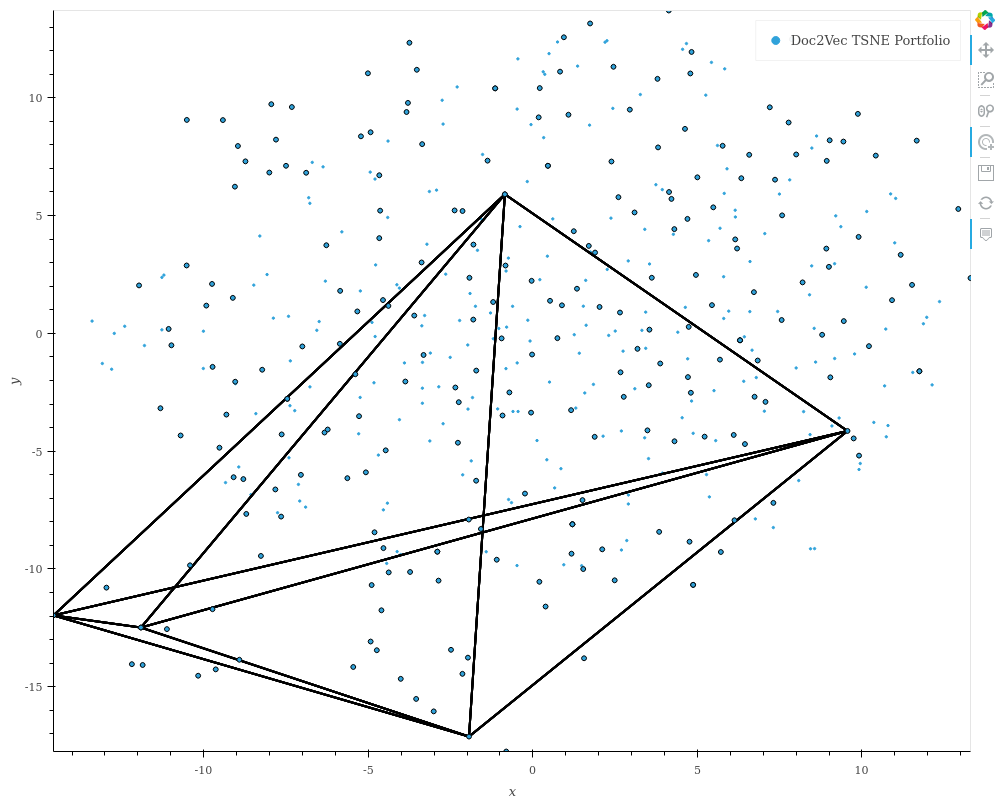
\includegraphics{../experiments/media/Association Computation Diagram.png}\\

\textbf{Figure 2: Association Computation Diagram}

\hypertarget{benchmarking}{%
\subsection{Benchmarking}\label{benchmarking}}

When compared to similar techniques in NLP the joint use of
Term-Frequency Inverse-Document-Frequency Weighting (TFIDF) and the
Word2Vec algorithm provide clear advantages in computational efficiency,
interpretability, and scalability. Algorithms such as Latent Semantic
Indexing (LSI), Latent Dirichlet Allocation (LDA) and Doc2Vec require
large matrix factorization, human interpretation, labeling and issues in
term-weighting adding to the bias and difficulty in their use. These
algorithms have been benchmarked in Appendix D against a dataset of
company descriptions using t-distributed Stochastic Neighbour Embedding
(tSNE) and Scaling by Majorizing a Complicated Function (SMACOF) with
accompanying descriptions of these methods and their use. Even if these
methods are considered computational efficient they do not meet the
requirements or intuitions of most analysts and can be considered
inappropriate for this study. Definitions of the above mentioned
techniques can be found in Appendix E.

\hypertarget{experimental-design}{%
\subsection{Experimental Design}\label{experimental-design}}

Our experimental design makes use of Analysis of Covariance (ANCOVA) in
order to evaluate the relationship between Association and portfolio
volatility.

The variance sum rule allows us to compute portfolio variance based on
the variance and covariance of shares in a portfolio.

\[ \sigma_{p}^{2} = \sum_{i}^{n} \sigma_{i}^{2} + \sum_{i,j=1, i \ne j}^{n} \sigma_{i} \sigma_{j} cov_{i,j} \]

In this formula, we specify \(n\) to be the number of shares in a
portfolio, \(\sigma_{p}\) to be the variance of the portfolio,
\(\sigma_{i}\) and \(\sigma_{j}\) to be the variance of shares \(i\) or
\(j\) in a given portfolio and \(cov_{i,j}\) to be the covariance
between shares \(i\) and \(j\) in the portfolio.

While shares may exhibit particular variance properties as a function of
their capital structure and operations, key in understanding the
diversification of a portfolio is the ability to quantify the
\(\Sigma_{i,j=1, i \ne j}^{n} \sigma_{i} \sigma_{j} cov_{i,j}\) term.

In order to compare our forward-looking portfolio volatility to
historical Association Risk we will look to evaluate the relationship
between the
\(\Sigma_{i,j=1, i \ne j}^{n} \sigma_{i} \sigma_{j} cov_{i,j}\) of the
Variance Sum Rule to our computed \(\text{Association}\). In order to do
this we specify a model for evaluating this hypothesis using the
following relationship:

The aim of diversification is to reduce the risk of a given portfolio,
for a given level of return:\\
\[\text{risk}_{p} \propto \frac{1}{\text{Diversification}_{p}} \]

According to the Variance Sum Rule:
\[ \sigma_{p}^{2} = \sum_{i}^{n} \sigma_{i}^{2} + \sum_{i,j=1, i \ne j}^{n} \sigma_{i} \sigma_{j} cov_{i,j} \]

The aim of diversification is to include shares of different covariances
to lower the risk in \(\sigma_{p}\). The Variance Sum Rule represents
diversification through the term:\\
\[ \sum_{i,j=1, i \ne j}^{n} \sigma_{i} \sigma_{j} cov_{i,j} \]

In this paper we Hypothesize \(\text{Association}_{p}\) as a measure
proportional to the level of diversification of a given portfolio, such
that using the Variance Sum Rule:\\
\[ \Sigma_{i,j=1, i \ne j}^{i,j \in p} \sigma_{i} \sigma_{j} cov_{i,j} \propto \text{Association}_{p}\]

When combining these formulas, substituting back into the Variance Sum
Rule, we get:
\[ \sigma_{p}^{2} = \sum_{i}^{n} \sigma_{i}^{2} + \sum_{i,j=1, i \ne j}^{n} \sigma_{i} \sigma_{j} cov_{i,j}  = \sum_{i}^{n} \sigma_{i}^{2} + f(\text{Association}_{p}) \]

Using this relationship, we can establish a model:\\
\[ \sigma_{p}^{2} = \beta_{0} + \beta_{1} \text{Association}_{p} + \Sigma_{i \in P} \beta_{i}\]

Where \(P\) are the items in a given portfolio. Which allows us to
appropriately control for share-specific volatility, to determine:\\
\[\text{Diversification}_{p} \propto \text{Association}_{p}\]

Using the Student's T-test, we can investigate the relationship between
our Association Risk metric and diversification, under the Null
Hypothesis:\\
\[\beta_{1} = 0\]

If, \[\beta_{1} = 0\]\\
Then no relationship exists between our Association Risk metric and the
diversification of our portfolio. However, if: \[\beta_{1} \ne 0\]

Then, \[\text{Diversification}_{p} \propto \text{Association}_{p}\]\\
Allowing investors to use Association Risk as an accurate measure of
portfolio risk.

ANCOVA will be used to test this hypothesis under the assumption of
normally distributed errors. ANCOVA examines the influence of an
independent variable on a dependent variable while removing the effect
of the covariate factor. It assumes a linear relationship between the
dependent variable and the covariate factor. Given the use of continuous
testing a time series plot of ANCOVA coefficients and p-values will be
used to analyze the relationship between Association and volatility.

\[ y_{i, j} = \mu + \tau_{i} + \beta (x_{i,j} - \bar{x}) + \epsilon_{i, j} \]

\begin{itemize}
\tightlist
\item
  \(Y_{i, j}\) is the covariate factor
\item
  \(u\) is the grand mean
\item
  \(x\) bar is the global mean\\
\item
  \(x_{i, j}\) is the jth observation of the jth covariate factor\\
\item
  \(t_{i}\) is the variables fitted\\
\item
  \(e_{i, j}\) is the error term.
\end{itemize}

This was tested for given portfolios across time, using the equation:

\[ \sigma_{p,t}^{2} = \beta_{0} + \beta_{1} \text{Association}_{p, t}) + \Sigma_{i \in P} \beta_{i}\]

In which a distribution of p-values is presented corresponding to the
Null hypothesis of \(\beta_{1, p} = 0\) for every portfolio, \(p\), in
our study. Next ANCOVA is used to test the Null Hypothesis,
\(\beta_{1} = 0\) across all our portfolios controlling for the
volatility of shares in a given portfolio and for changes in mean market
volatility over time using the equation:

\[ \sigma_{p,t}^{2} = \beta_{0} + \beta_{1} \text{Association}_{p,t} + \beta_{t} + \Sigma_{i \in P} \beta_{i} \]

\newpage

\hypertarget{results-and-discussion}{%
\section{Results and discussion}\label{results-and-discussion}}

\hypertarget{news-volume-and-association}{%
\subsection{News volume and
association}\label{news-volume-and-association}}

In analyzing news volume over time it is clear that the volume of news
articles scraped before 2009 is extremely low. Figure 3 details word
vector associations over time. These seem to appear completely constant,
only displaying variance from 2008 onwards. This is due to the number of
news articles used increasing dramatically during this period which
remains a limitation of this study. Figure 4 details the volume plot and
is related to the association plot in that as news article volume
increases so does the stability and accuracy of word vectors used to
compute Association.

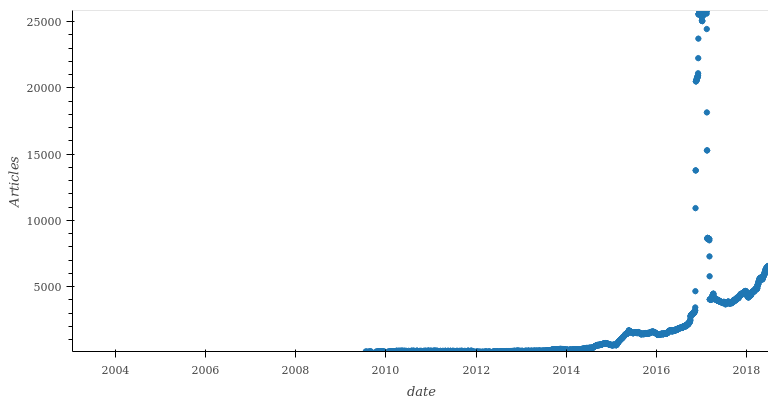
\includegraphics{../experiments/media/News Volume.png}\\

\textbf{Figure 3: News Volume}

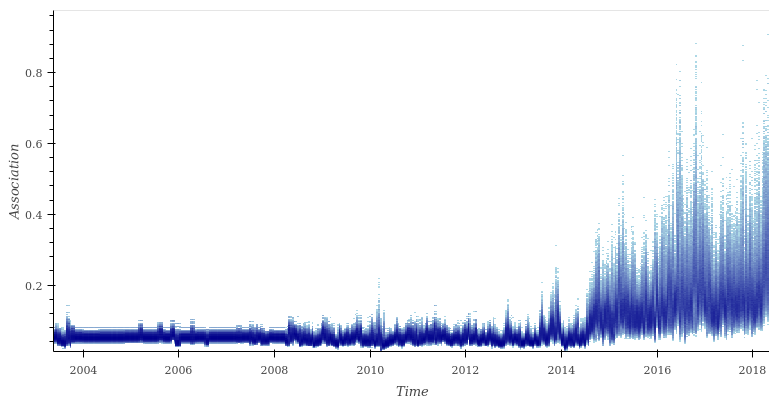
\includegraphics{../experiments/media/Association Over Time.png}\\

\textbf{Figure 4: Association}

Volatility details the standard deviation of portfolios over time.
Figure 5 shows the 300-day volatility of returns across 1000 random
evenly weighted portfolios between 16 May 2003 and 17 May 2018. When
assessing volatility over time the influence of macroeconomic events
such as the financial crisis in 2008 and the South African ``Zuma-gate
scandal'' of 2016 are attributed to the spikes in portfolio volatility.

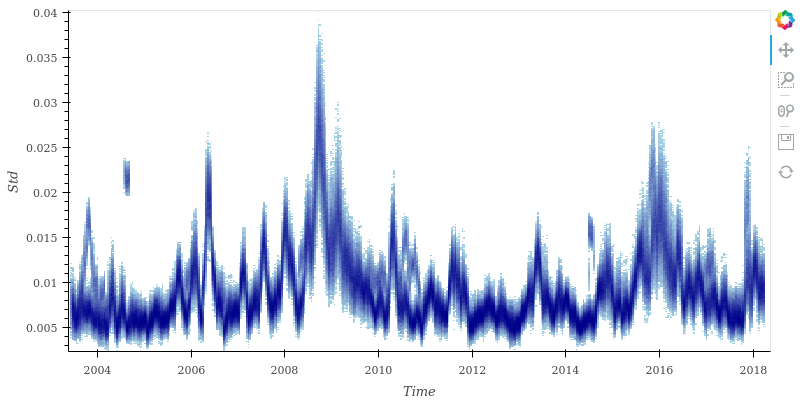
\includegraphics{../experiments/media/Volatility Over Time time.png}\\

\textbf{Figure 5: Volatility}

Portfolios comprise of many sources of volatility which arise due to
market microstructure, market events and the inclusion of particular
shares with high long-run volatility characteristics. In order to
explore the relationship between association and portfolio volatility we
propose the analysis of single portfolios over time. By analyzing
portfolios on an individual basis, we hope to control for long-run
company specific volatility characteristics, whilst avoiding the
overparameterization of our model.

In this model, we assume the \$ \sum\emph{\{i=1\}\^{}\{n\}
\sigma}\{i\}\^{}2 \$ term in the Variance Sum Rule to be included as
come constant term, \(\beta_{0}\), allowing for the direct comparison
between Association Risk and portfolio volatility. This method, which we
will refer to as ``Portfolio ANCOVA'', relies on a key assumption, that
\(\Sigma_{i,j=1, i \ne j}^{n} \sigma_{i} \sigma_{j} cov_{i,j}\) serves
as the primary driver of portfolio risk over time. As this term serves
as a function of variance, covariance and their interaction, it includes
all critical factors in relating portfolio diversification to
Association Risk in a manner which is computationally efficient and
ideal for our analysis.

\hypertarget{portfolio-ancova}{%
\subsection{Portfolio ANCOVA}\label{portfolio-ancova}}

In Figure 10, it is clear that the coefficient on Association Risk is
normally distributed and lies in a reasonable range of positive values,
which suggests that there is significance in the model. The same can be
said for the ANCOVA constant x-values which exhibit similar traits, in
Figure 11. The coefficient p-value plot, in Figure 9 of the Appendix,
shows that the coefficient on Association Risk for a given portfolio
across time is significant at the 0.1\% level with a small minority of
portfolios significant at the 0.5\% level. This is sufficient evidence
to reject the null hypothesis and conclude that \(\beta_{1}\) is not
equal to 0. If \(\beta_{1}\) is not equal to 0, a relationship exists
between Association Risk and Portfolio Volatility, presenting evidence
for its use as a predictor of portfolio diversification and our
hypothesis in this study.

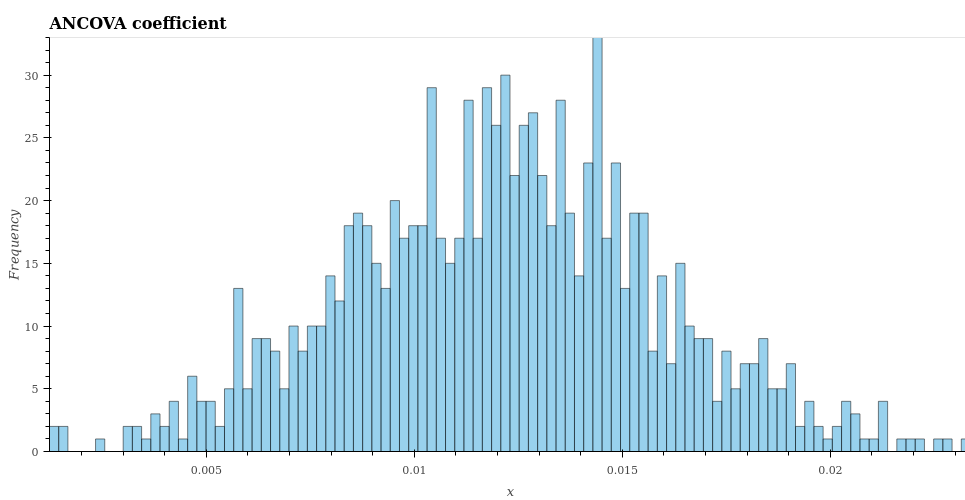
\includegraphics{../experiments/media/Coefficeint value with constant accross portfolio.png}\\

\textbf{Figure 10: Coefficients Across Time Within Portfolios}

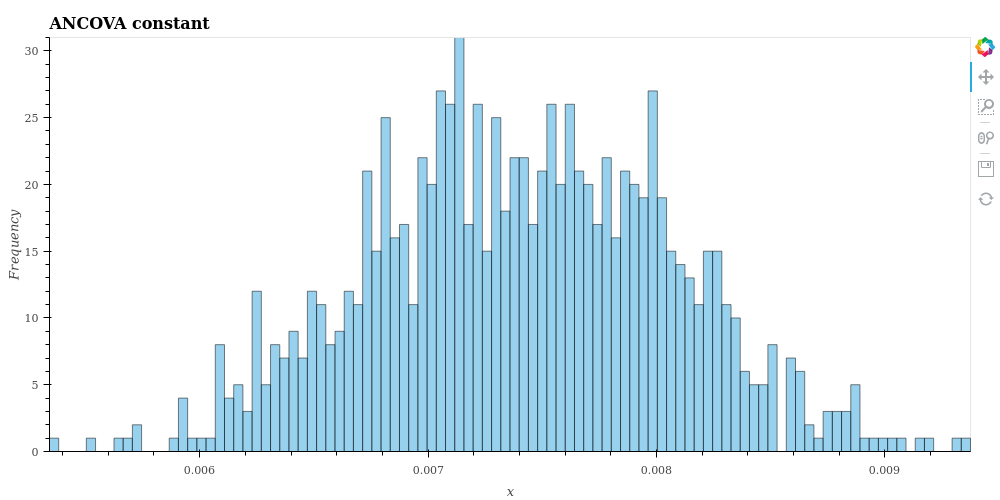
\includegraphics{../experiments/media/Constant value with constant accross portfolio.png}

\textbf{Figure 11: Constants Across Time Within Portfolios}

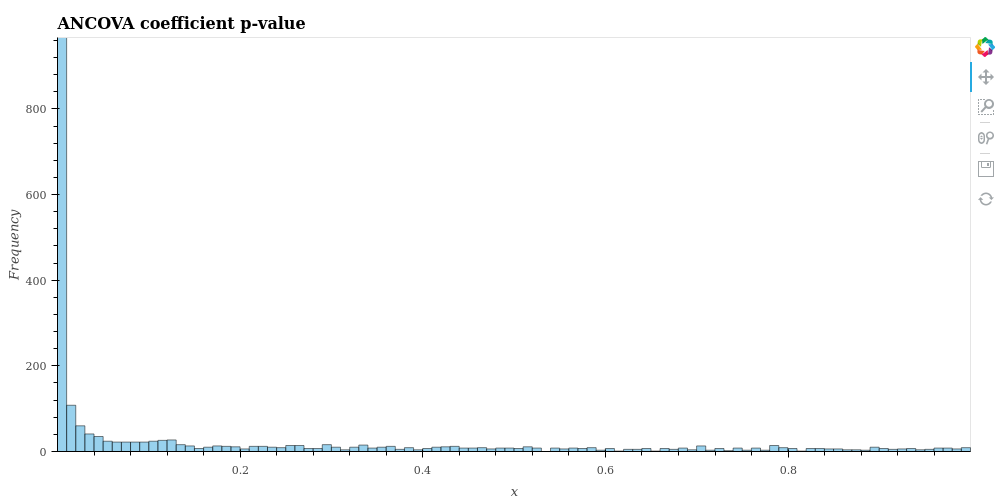
\includegraphics{../experiments/media/Coefficeint P-value with contant accross portfolio.png}\\

\textbf{Figure 12: Coefficient P-values Across Time Within Portfolios}

In order to understand why these results may be significant we analyze
the distribution of a single portfolio over time, looking at the 500th
portfolio to assess Association and its relationship to portfolio
volatility. Despite the long-tail distribution of volatility, Figure 13
demonstrates a clear positive relationship between Association Risk and
portfolio volatility. While the distribution of Association Risk
obscures the presence of heteroskedasticity, the simplicity and
under-parameterization of this model suggests that Association Risk
finds poor application as the sole predictor of volatility, without
controlling for market events and short-term company-specific volatility
characteristics.

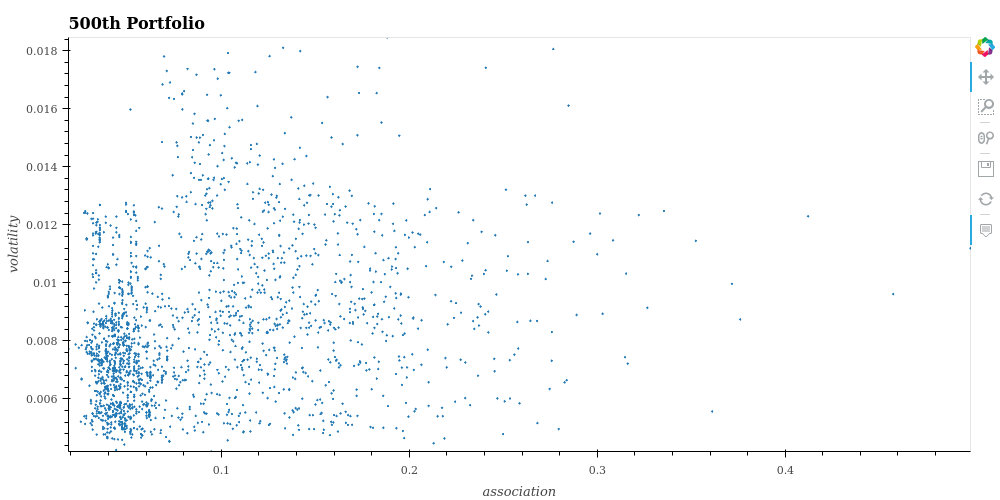
\includegraphics{../experiments/media/Scatter Plot of 500th Portofolio.png}\\

\textbf{Figure 13: Scatter Plot of Association and Volatility of the
500th Portfolio}

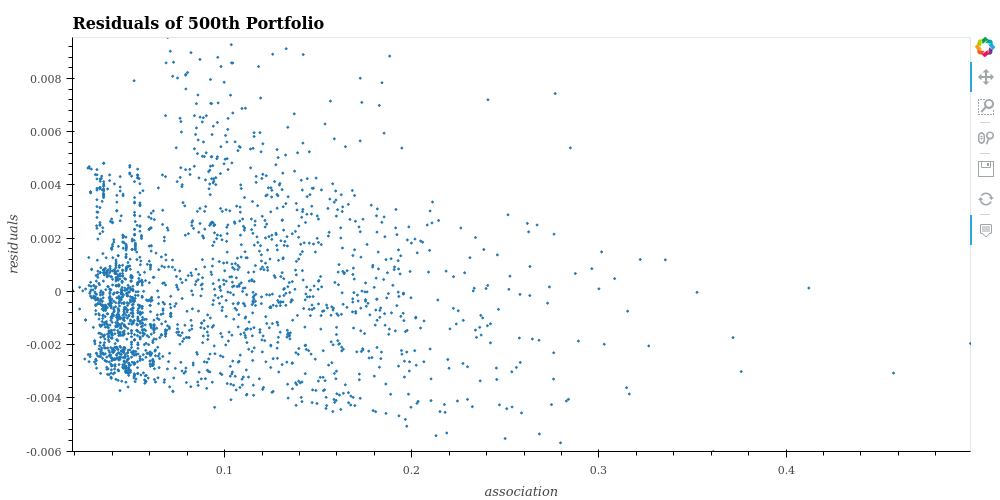
\includegraphics{../experiments/media/Scatter Plot of Residuals of 500th Portofolio.png}\\

\textbf{Figure 14: Scatter Plot of Association and Residuals of the
500th Portfolio}

\newpage

\begin{longtable}[]{@{}llll@{}}
\toprule
& \textbf{Table 3} & &\tabularnewline
\midrule
\endhead
Dep. Variable & y & R-squared & 0.068\tabularnewline
Method: & Least Squares & Adj. R-squared & 0.068\tabularnewline
No.~Observations: & 2058 & F-statistic & 150.8\tabularnewline
DF Residuals: & 2056 & Prob(F-statistic) & 1.70e-33\tabularnewline
Df Model: & 1 & Log-likelihood & 9334.1\tabularnewline
Covariance type & non-robust & AIC: & -1.866e+04\tabularnewline
& & BIC: & -1.865e+04\tabularnewline
& & &\tabularnewline
& Coef & std err & t\tabularnewline
constant & 0.0075 & 0.000 & 72.687\tabularnewline
X1 & 0.0114 & 0.001 & 12.279\tabularnewline
& & &\tabularnewline
& p\textgreater{}\textbar{}t\textbar{} & {[}0.025 &
0.975{]}\tabularnewline
constant & 0.000 & 0.007 & 0.008\tabularnewline
X1 & 0.000 & 0.010 & 0.013\tabularnewline
& & &\tabularnewline
\bottomrule
\end{longtable}

\newpage

\hypertarget{incorporation-of-time-blocking}{%
\subsection{Incorporation of Time
Blocking}\label{incorporation-of-time-blocking}}

Through an analysis in Portfolio ANCOVA this paper has identified the
many sources of portfolios variation. We conclude the two main sources
of variance to be excess systematic volatility on a given day and excess
volatility of a particular share in a portfolio. We propose a second
method in which to control for these sources of variance using blocking.

Using data on shares in our portfolios we propose a model to test for
these sources of variation jointly, shown in the equation below:\\
\[ \sigma_{p,t}^{2} = \beta_{0} + \beta_{1} \text{Association}_{p,t} + \beta_{t} + \Sigma_{i \in P} \beta_{i} \]

Where \(t\) represents a trading day in our dataset and \(P\) represents
a set of companies in a given portfolio.

Given the number of data points, a stratified sampling of our data was
taken in order to fit this model using the Ordinary Least Squares
method. The results are shown in the table below:

/newpage

\begin{longtable}[]{@{}llll@{}}
\toprule
& \textbf{Table 4} & &\tabularnewline
\midrule
\endhead
Dep. Variable & y & R-squared & 0.794\tabularnewline
Method: & Least Squares & Adj. R-squared & 0.790\tabularnewline
No.~Observations: & 123450 & F-statistic & 182.6\tabularnewline
DF Residuals: & 120899 & Prob(F-statistic) & 0.000\tabularnewline
Df Model: & 2550 & Log-likelihood & 6.2152e+05\tabularnewline
Covariance type & non-robust & AIC: & -1.238e+64\tabularnewline
Date & Mon, 17 Sep 2018 & BIC: & -1.213e+06\tabularnewline
Time & 23:56:13 & &\tabularnewline
& & &\tabularnewline
& Coef & std err & t\tabularnewline
Association & 0.007 & 0.000 & 3.529\tabularnewline
\ldots{} & & &\tabularnewline
Constant & 0.0024 & 4.84e-06 & 500.510\tabularnewline
& & &\tabularnewline
& p\textgreater{}\textbar{}t\textbar{} & {[}0.025 &
0.975{]}\tabularnewline
Association & 0.000 & 0.000 & 0.001\tabularnewline
\ldots{} & & &\tabularnewline
Constant & 0.000 & 0.002 & 0.002\tabularnewline
& & &\tabularnewline
Omnibus: & 25356.151 & Skew: & 0.933\tabularnewline
Prob(Omnibus): & 0.000 & Kurtosis: & 7.402\tabularnewline
Prob(JB): & 0.000 & Cond. No. & 1.72e+17\tabularnewline
& & &\tabularnewline
Dubin-Watson & 1.999 & &\tabularnewline
Jarque-Bera (JB): & 117583.806 & &\tabularnewline
& & &\tabularnewline
\bottomrule
\end{longtable}

\newpage

From the 120899 observations we can observe a constant value of 0.0024
and an Association coefficient of 0.0007, both of which are significant
at the 0.1\% level, with t-scores of 500.510 and 3.529 respectively.
This model demonstrates a \(R^2\) value of 0.794 and joint-significance
of 182.6 which is significant at the 0.1\% level using Fisher's
F-statistic. If we then analyze the residuals of this model, shown in
Figure 15, we observe their distribution as both symmetric and
distributed around 0 with little correlation to Association as shown in
Figure 15. These properties are crucial to the Gauss-Markov Assumptions
of Ordinary Least Squares Linear Regression and the use of these
estimates as an unbiased linear estimator of portfolio variance. The
p-values of our date coefficient under the null hypothesis
\(\beta_{t} = 0\) are both significant and insignificant at points in
time, suggesting the effect of exogenous shocks to our model as shown in
Figure 17. Despite these findings we see using blocking to control for a
share's excess volatility demonstrating significant p-values at the
0.001\% level using the student t-distribution, providing a strong
argument for their use in this blocking design as shown in Figure 18.

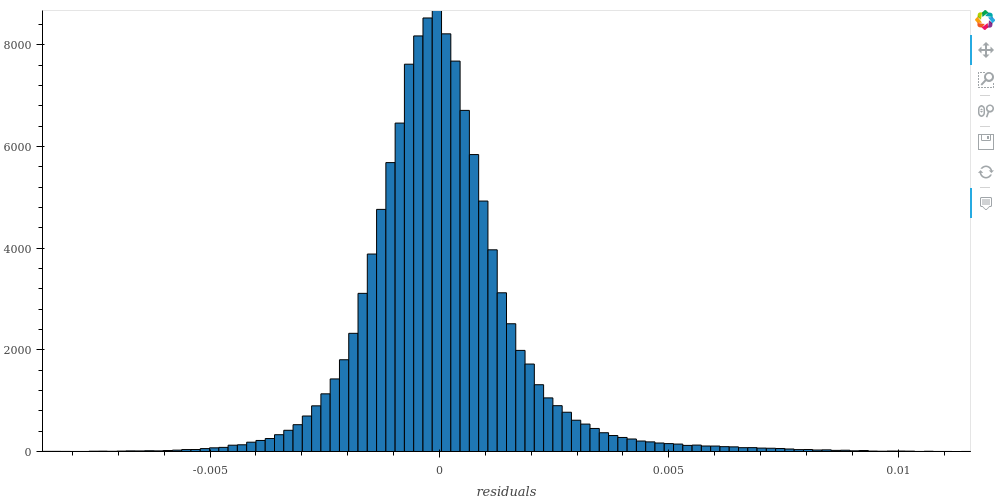
\includegraphics{../experiments/media/Histogram of Residuals of Blocking Ancova.png}\\

\textbf{Figure 15: Histogram of Residuals for the Blocking ANCOVA}

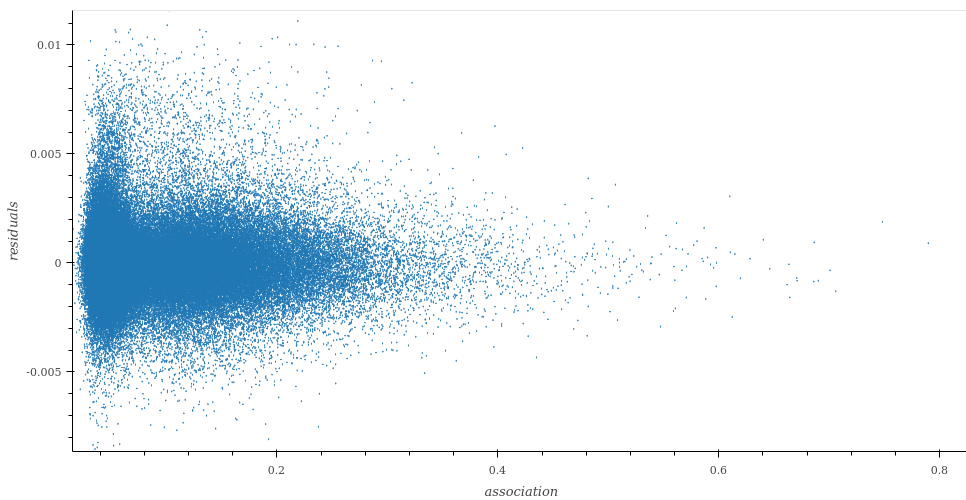
\includegraphics{../experiments/media/Scatter Plot of Residuals of Blocking Ancova.png}\\

\textbf{Figure 16: Scatter Plot of Association and Residuals Blocking
ANCOVA }

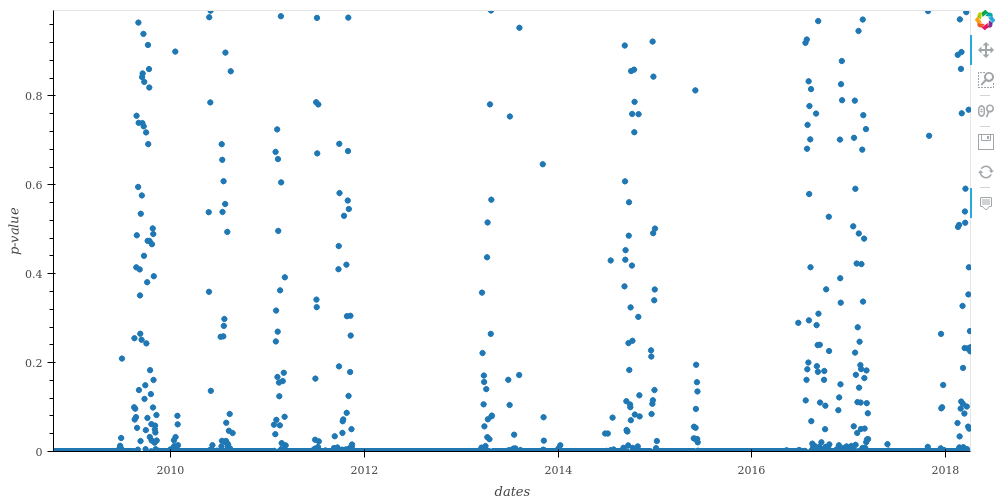
\includegraphics{../experiments/media/Scatter Plot of P-values for dates of Blocking Ancova.png}\\

\textbf{Figure 17: Scatter Plot of P-values for Dates of Blocking
ANCOVA}

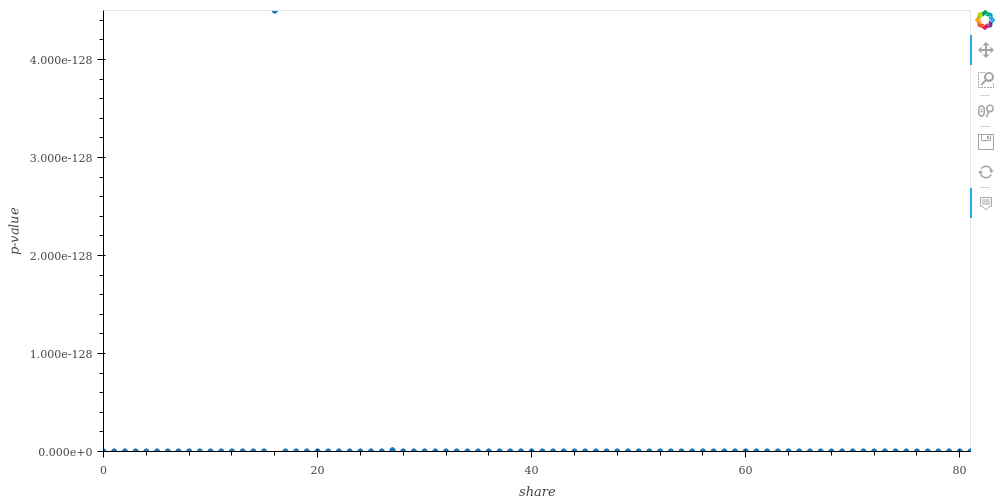
\includegraphics{../experiments/media/Scatter Plot of P-values for shares in a portfolio of Blocking Ancova.png}\\

\textbf{Figure 18: Scatter Plot of P-values for Portfolios of Blocking
ANCOVA}

\newpage

\hypertarget{conclusion}{%
\section{Conclusion}\label{conclusion}}

Whilst the Capital Asset Pricing Model (CAPM) remains at the foreground
of financial theory, empirical evidence suggests it is unreliable in
markets which exhibit low forms of efficiency. In inefficient markets
investors are unable to achieve perfect diversification and as a result,
may be subject to additional sources of non-systematic risk not
predicted by the CAPM. This paper provides investors with an alternative
risk metric known as Association Risk which offers investors a way in
which to determine the level of diversification of a given portfolio
without relying on inefficient price data. Using Association Risk,
investors can evaluate portfolio diversity using qualitative data.
During periods of extreme inefficiency prices no longer incorporate all
public or private information in the market. If investors assume
time-homogeneity in the statistical properties between shares over time
in order to make investment decisions, the price inefficiencies render
these assumptions inappropriate in evaluating medium and long-term
portfolio risk. Using Association Risk investors can incorporate
information directly to evaluate the risk of a given portfolio in
situations where price is misleading for continued risk management in
times of crisis.

This paper suggests the use of document vectors as accurate and unbiased
measures of firm-specific characteristics in identifying a holistic,
unbiased and dynamic measure for use in determining non-systematic
primary risk factors for use in portfolio construction. This metric
provides a smooth and continuous mapping between companies and their
industry or similarity to one another which goes beyond simple
identification of ``core-business'' as used in the literature.

The relationship between the Association of shares within a portfolio on
the Johannesburg Stock Exchange (JSE) and portfolio volatility is
confirmed by the results of this study. Firstly, using ``Portfolio
ANCOVA'' this paper is able to isolate the effects of Association on
volatility over time and produce significant results. Whilst we are
confident that covariance is not equal to zero, the extent to which the
coefficients vary implies Association Risk inappropriate for use in
predictive applications. Secondly, using a blocking experimental design,
this paper finds strong evidence in identifying the relationship between
Association and portfolio variance when controlling for excessive
systematic variance at points in time and contributions of variance by
outlying high volatility shares.

An opportunity for future research exists in which Association Risk
could be used in predictive modeling, exploratory analysis, portfolio
optimization and risk-characterization across indexes. Using this tool
researchers may be able to better quantify market efficiency over time
and develop existing methodologies for improved application in
developing markets.

\newpage

\hypertarget{appendix}{%
\section{Appendix}\label{appendix}}

\hypertarget{appendix-a}{%
\subsection{Appendix A}\label{appendix-a}}

\hypertarget{tf-idf}{%
\subsubsection{TF-IDF}\label{tf-idf}}

TF-IDF is an information retrieval technique that weighs a term's
frequency (TF) and its inverse document frequency (IDF). Each term has
its respective TF and IDF score and the product of the scores is the
TF-IDF weight of that term. The higher the score the rarer the term and
vice versa. This score is used to assign the importance of the term
throughout the corpus. For a term, \(t\) in document, \(d\), the weight
Wt,d of term t in document d is given by:

\(W_{t,d} = TF_{t,d} log(N/DF_{t})\)

Where:\\
- \(TF_{t,d}\) is the number of occurrences of \(t\) in document
\(d\).\\
- \(DF_{t}\) is the number of documents containing the term \(t\).\\
- \(N\) is the total number of documents in the corpus.

\hypertarget{word2vec}{%
\subsubsection{Word2Vec}\label{word2vec}}

A simplified explanation of Word2Vec is that it figures out how to place
words on a ``chart'' in such a way that their location is determined by
their meaning, called a vector-space. This means that words with similar
meanings will be clustered together. I.e.: Words with semantic
relationships will be closer together than words without such
relationships. Word2Vec is a three-layer neural network with one input,
one hidden and an output layer. Word2Vec can utilize Continuous bag of
words (CBOW) or continuous skip-gram architecture. The idea of CBOW
(continuous bag-of-words) architecture, the Word2Vec algorithm we are
using, is to learn word representations that can predict a word given
its surrounding words. The input layer corresponds to signals for
surrounding words and output layer correspond to signals for a predicted
target word. Suppose, you have an input sentence: ``The cat sat on the
mat''. The aim is to learn representation for words ``the'', `'cat'',
``sat'' etc. To this end, the neural network tries to learn features
(weights W and W') which look at words in a window, say ``The cat sat''
and try to predict the next word, ``on''. Hence, with input as the
``the'', `'cat'', `'sat'', the training process adjusts the weight of
the network, so that the probability of output ``on'' is maximized, as
compared to other words in the vocabulary. As the training procedure
repeats this process over a large number of sentences or phrases, the
weights ``stabilize''. These weights are then used as the vectorized
representations of words.

\hypertarget{word2vec-diagrams}{%
\subsubsection{Word2Vec Diagrams}\label{word2vec-diagrams}}

\begin{figure}
\centering
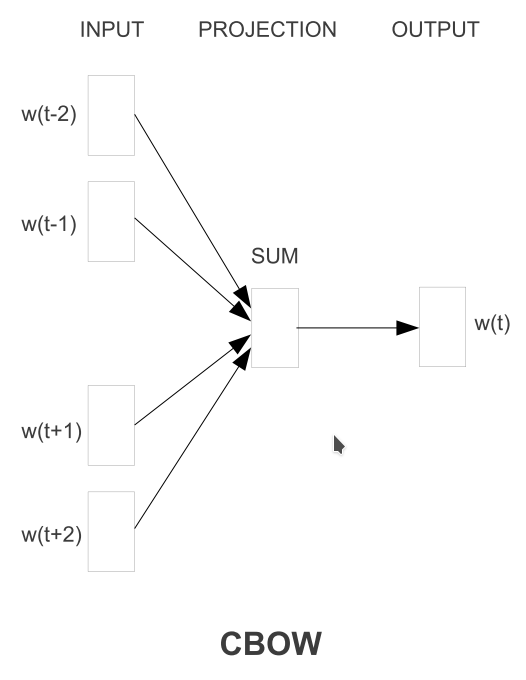
\includegraphics{../experiments/media/Word2Vec CBOW.png}
\caption{Word2Vec CBOW}
\end{figure}

{[}@Mikolov2013a{]}

The CBOW architecture predicts the current word based on the context of
a given word.

\begin{figure}
\centering
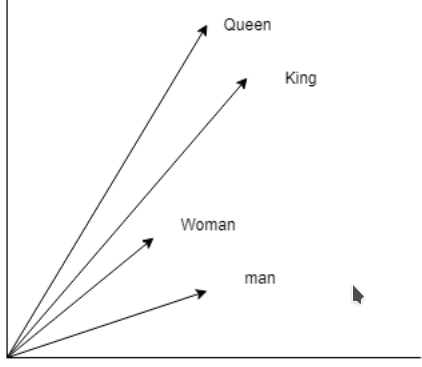
\includegraphics{../experiments/media/Word2vec simplified.png}
\caption{Simplified Word2Vec}
\end{figure}

This diagram outlines the vector relationship maintained through the use
of word embeddings.\\
king - man + woman = queen

\hypertarget{negative-sampling}{%
\subsubsection{Negative Sampling}\label{negative-sampling}}

Negative-sampling is a method by which samples are drawn outside a given
distribution. In the context of Word2Vec and Doc2Vec embedding
techniques, this involves sampling incorrect contexts for a given word
or incorrect document tags for a given document to be used as false
labels when training the embedding model.

\#\# Appendix B: Companies in the analysis

`ACL', `AEG', `AEL', `AFE', `AFX', `AGL', `AMS', `ANG', `APN', `ARI',
`ASR', `AVI', `AXL', `BAT', `BAW', `BGA', `BIL', `BVT', `CAT', `CLS',
`CML', `CPI', `DRD', `DST', `DSY', `DTA', `DTC', `EOH', `EXX', `FBR',
`FSR', `GFI', `GND', `HAR', `HCI', `IMP', `INL', `INP', `IPL', `KAP',
`LBH', `LON', `MMI', `MRF', `MRP', `MSM', `MTN', `MUR', `NED', `NHM',
`NPK', `NPN', `NTC', `OCE', `OML', `OMN', `PBG', `PIK', `PPC', `PSG',
`RCL', `REM', `RLO', `RMH', `SAP', `SBK', `SHP', `SLM', `SNH', `SNT',
`SOL', `SPG', `SUI', `TBS', `TFG', `TKG', `TON', `TRE', `TRU', `TSH',
`WBO' and `WHL'.

\hypertarget{appendix-c-news-sources}{%
\subsection{Appendix C: News Sources}\label{appendix-c-news-sources}}

\begin{longtable}[]{@{}ll@{}}
\toprule
Number of Articles Sources & Source\tabularnewline
\midrule
\endhead
88 & biznews\tabularnewline
63513 & businesslive\tabularnewline
146 & entrepreneurmag\tabularnewline
77492 & fin24\tabularnewline
18884 & financialmail\tabularnewline
44 & iafrica\tabularnewline
38262 & iol\tabularnewline
100 & mg\tabularnewline
9780 & moneyweb\tabularnewline
16439 & timeslive\tabularnewline
224748 & \textbf{total}\tabularnewline
\bottomrule
\end{longtable}

\hypertarget{appendix-d-exploratory-data-analysis}{%
\subsection{Appendix D: Exploratory data
analysis}\label{appendix-d-exploratory-data-analysis}}

A number of techniques remain popular within the literature of NLP.
These include LDA, LSI, Doc2Vec and Word2Vec amongst others. In the
following section we analyze these four techniques and aim to visualize
their data in order to assess their power in drawing association between
companies on the JSE.

Models are first trained on a fixed dataset of company descriptions.
Document vectors are then computed using these various models
representing each company. Two techniques were used in order to
visualize these 100-dimensional document vectors, namely t-distributed
Stochastic Neighbour Embedding (tSNE), a popular manifold embedding
technique, and Scaling by Majorizing a Complicated Function (SMACOF), a
self organizing map technique which uses a stress measure in order to
create a lower dimensional representation of data which maintains the
distances between document vectors. Word2Vec is computed using cosine
distances and Doc2Vec, LSI and LDA are computed using Euclidean
distances.

One challenge in interpreting techniques is in benchmarking adequate
tools for dimensionality reduction in order to visualize our
100-dimensional document vectors. This dimensionality reduction results
in some of the relationships between vectors being lost. For tSNE,
document vectors are most accurate in their immediate neighbourhood due
to the distributional assumption of the technique.

In Figure 1 and 2 a scatter plot is produced for all companies in our
corpus with random sampling of labels to aid in interpretation. If we
analyze the diagram, we see that telecommunications companies like
Vodacom and MTN grouped together, as well as mining companies like Gold
Fields and Glencore. A number of the insurance, property and finance
companies are also close in proximity. While many of the relationships
in the diagram are not easily explainable, given the size of the dataset
used, it is challenging for a reliable word-vector model to be estimated
without the use of techniques such transfer-learning.

When comparing Word2Vec against other techniques we see striking
differences, seen in Figures 3 to 8. The first of which is that in
techniques like LSI, we see far stronger clustering of companies with
similar names or similar attributes or description. This is largely
attributable to the underlying methodology in which a Bag-of-Words is
reduced to its dimensionality using some form of Principal Component
Analysis (PCA) with little concern for polysemy. While similar
limitations exist in techniques such as LDA, LDA Hierarchical Bayesian
Estimation also lacks sufficient variation to distinguish strongly
between companies.

When assessing Doc2Vec in figures 3 and 4 we see the problem of excess
noise from article words whose weighting cannot be reduced in the same
way TFIDF does with Word2Vec, as TFIDF provides more stable and accurate
word vectors is given the size of the corpus.

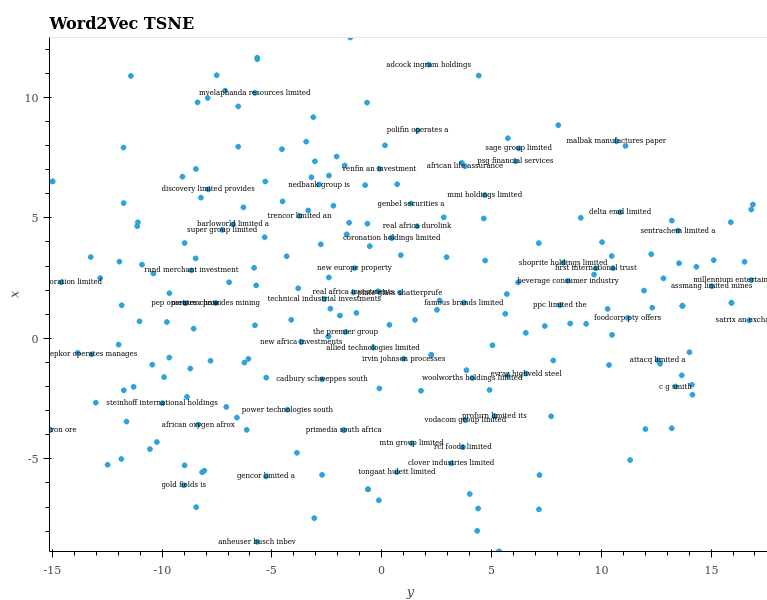
\includegraphics{../experiments/media/Word2Vec TSNE.png}\\

\textbf{Figure 1: Word2vec t-SNE}

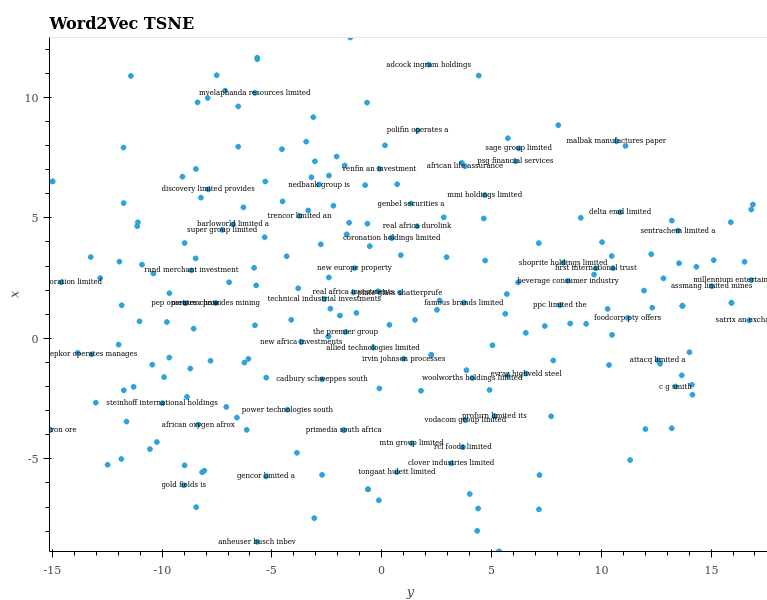
\includegraphics{../experiments/media/Word2Vec TSNE.png}\\

\textbf{Figure 2: Word2vec SMACOF}

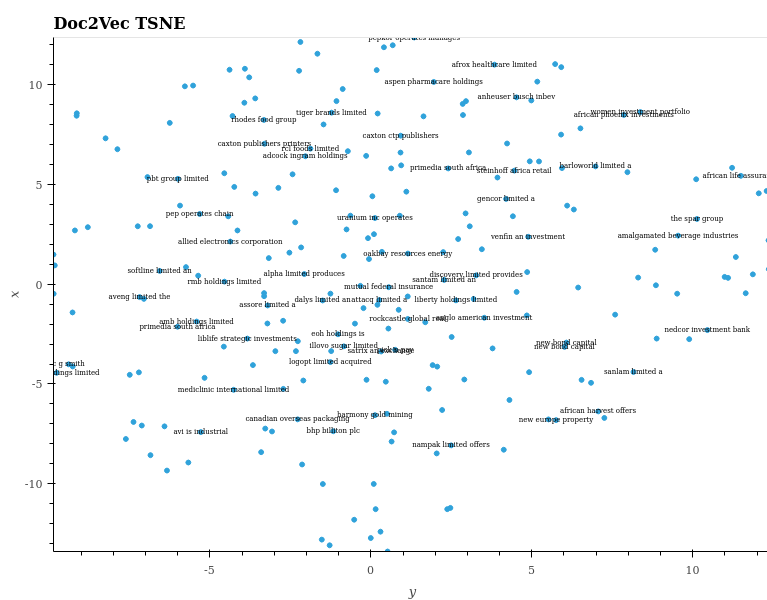
\includegraphics{../experiments/media/Doc2Vec TSNE.png}\\

\textbf{Figure 3: Doc2vec t-SNE}

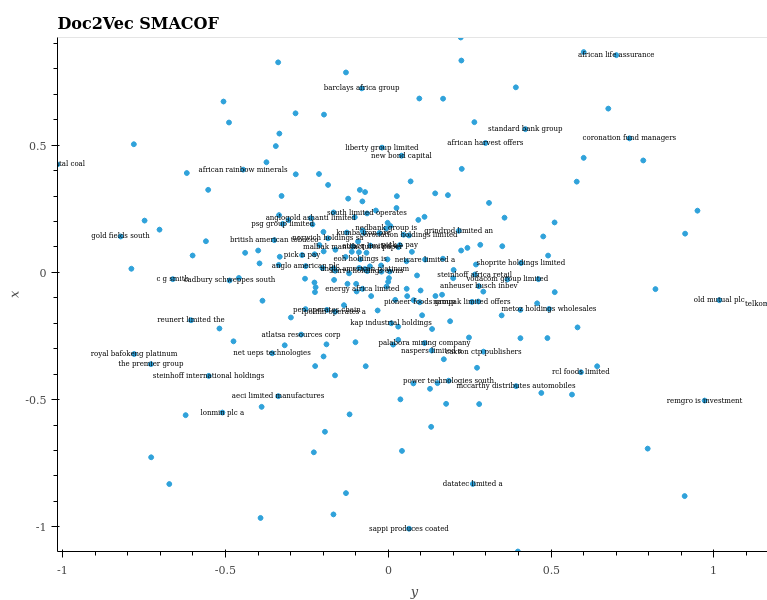
\includegraphics{../experiments/media/Doc2Vec SMACOF.png}\\

\textbf{Figure 4: Doc2vec SMACOF}

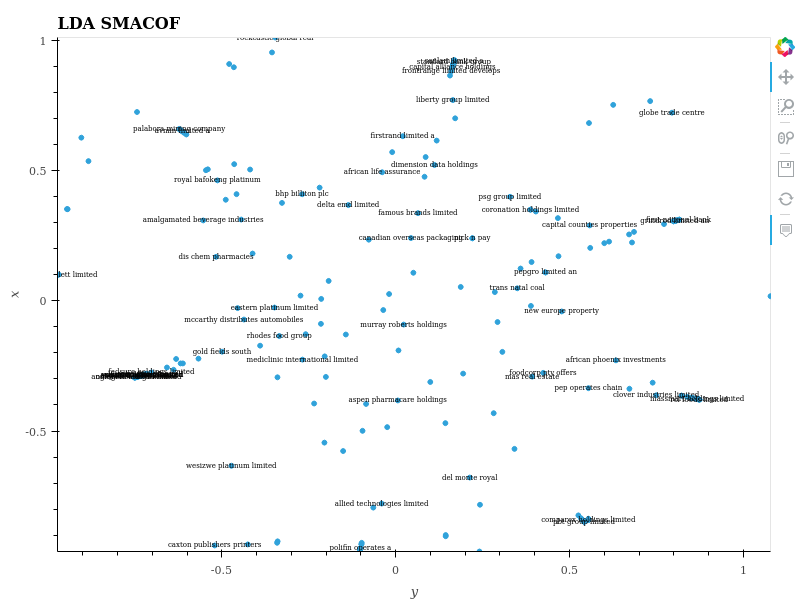
\includegraphics{../experiments/media/LDA SMACOF.png}\\

\textbf{Figure 5: LDA t-SNE}

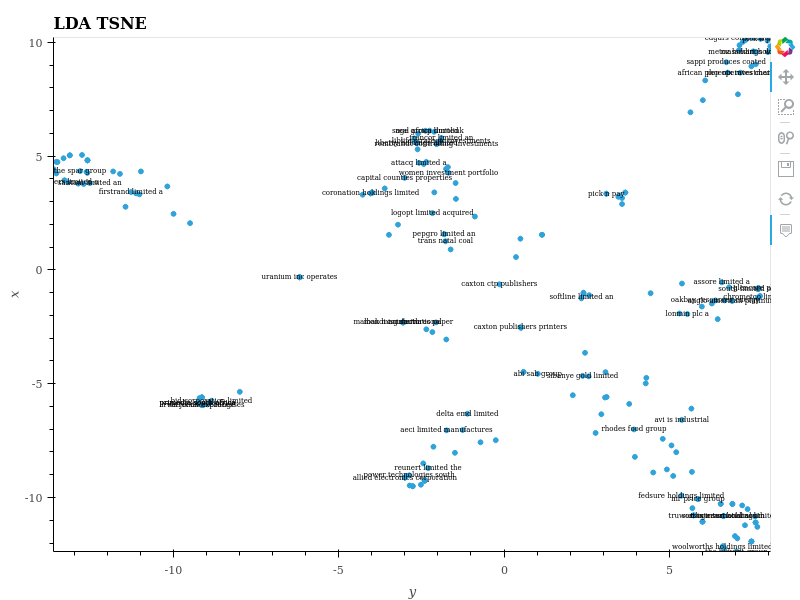
\includegraphics{../experiments/media/LDA TSNE.png}

\textbf{Figure 6: LDA SMACOF}

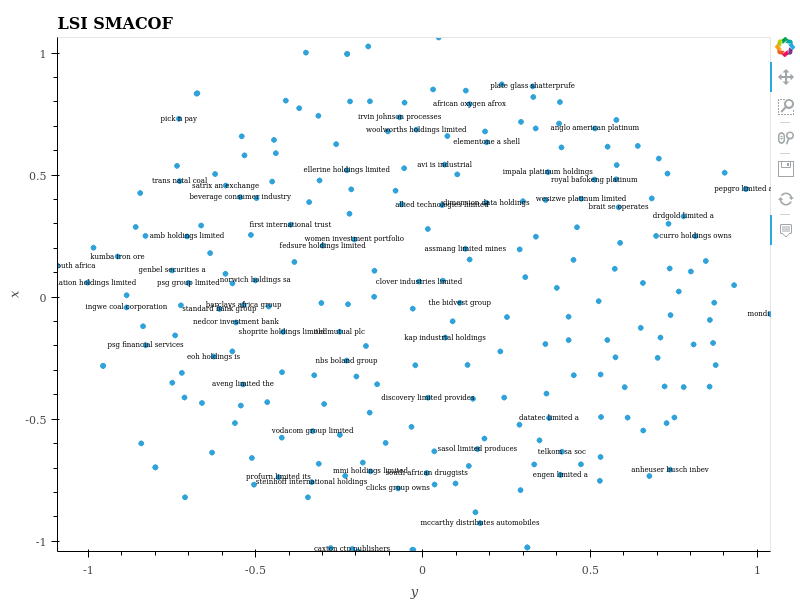
\includegraphics{../experiments/media/LSI SMACOF.png}\\

\textbf{Figure 7: LSI t-SNE}

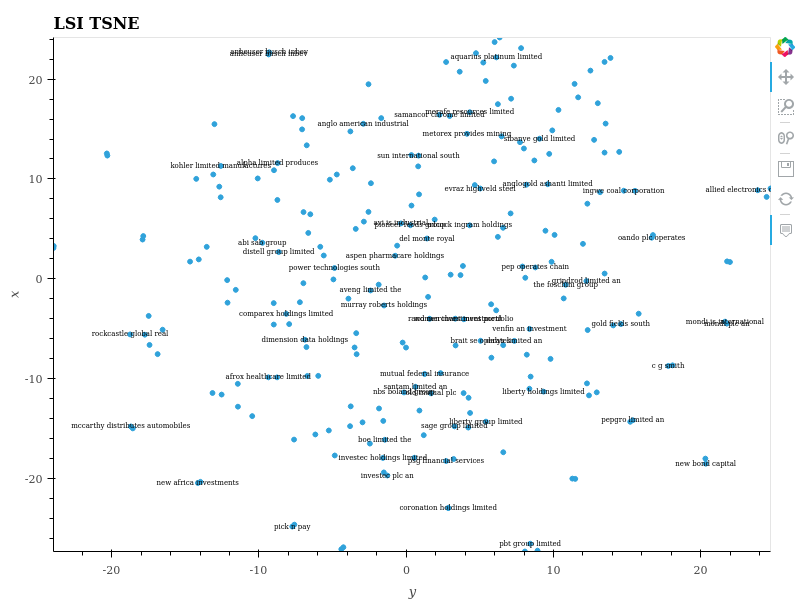
\includegraphics{../experiments/media/LSI TSNE.png}\\

\textbf{Figure 8: LSI SMACOF}

\hypertarget{appendix-e}{%
\subsection{Appendix E:}\label{appendix-e}}

\hypertarget{doc2vec}{%
\subsubsection{Doc2Vec}\label{doc2vec}}

Doc2Vec is an adaption of Word2Vec but instead of generating
relationships between words it generates relationships between
paragraphs, sentences, and documents. Again, there is a three-layer
neural network with an input, a hidden and an output layer. The
difference is that in the input layer there is now a signal for the
document as well as the signals for surrounding words which is what
makes the distinction between documents. The output layer, again,
corresponds to signals predicting target words.

\hypertarget{lda}{%
\subsubsection{LDA}\label{lda}}

Latent Dirichlet Allocation (LDA) is a generative statistical model that
allows sets of observations to be explained by unobserved groups that
explain why some parts of the data are similar. For example, an LDA
model might have topics classified as finance-related and
mining-related. Topics have probabilities of generating various words
such as ore, gold, strikes which can be classified and interpreted by
the viewer as mining-related. Likewise, the finance-related topic has
probabilities of generating words commonly associated with finance.
Words without relevance will have roughly equal probabilities. A lexical
word may occur in several topics with a different probability but with a
different typical set of neighboring words in each topic. Each document
is assumed to be characterized by a set of topics which makes the
individual words exchangeable.

\hypertarget{lsi}{%
\subsection{LSI}\label{lsi}}

Latent Semantic Indexing (LSI)is a technique of analyzing relationships
between a set of documents and the terms they contain by producing a set
of concepts related to the documents and terms. LSI assumes that words
that are close in meaning will occur in similar pieces of text. A matrix
containing word counts per paragraph is constructed from a large piece
of text and a mathematical technique called Singular Value Decomposition
is used to reduce the number of rows while preserving the similarity
structure among columns. Words are then compared by taking the cosine of
the angle between the two vectors formed by any two rows. Values close
to 1 represent very similar words while values close to 0 represent very
dissimilar words.

\hypertarget{smacof}{%
\subsubsection{SMACOF}\label{smacof}}

\[ \sigma(X) = \sum_{i<j<n} w_{i,j} (d_{i,j}(X)-\delta_{i,j})^2 \]

SMACOF uses an algorithm called majorizing to minimize stress functions.
Strictly speaking, majorization is not an algorithm but rather an
approach to constructing optimization algorithms. The principle of
majorization is to construct a surrogate function which
majorizes/minimizes a particular function. In some optimizations
problems, the objective-function is just too complicated to evaluate
directly at every iteration. Surrogate functions are constructed to
mimic most of the properties of the true objective-function, but that is
much simpler analytically and/or computationally.

\hypertarget{tsne}{%
\subsubsection{TSNE}\label{tsne}}

t-distributed stochastic neighbor embedding (t-SNE)

t-SNE is a tool to visualize high-dimensional data. It converts
similarities between data points to joint probabilities and tries to
minimize the Kullback-Leibler divergence between the joint probabilities
of the low-dimensional embedding and the high-dimensional data. t-SNE
has a cost function that is not convex, i.e.~with different
initializations we can get different results.

\newpage

\hypertarget{references}{%
\section{References}\label{references}}


    % Add a bibliography block to the postdoc
    
    
    
    \end{document}
